\chapter{Anti-unification of a pair of AUASTs} \label{ch4} \label{methodology}
\NZ{I would be grateful if you could help me to choose an appropriate title for this chapter. It describes my approach to construct anti-unifier, its implementation, and the experiment I conducted to evaluate it.}


\RW{Lots of this stuff is now moved to earlier chapters.  This chapter needs to be reworked as a result.  It's not clear to me that "chapter3-2.tex" needs to be separate from this.}
\RW{New intro blurb needed. Basically, you need to point out how Jigsaw does not suffice, which hopefully you will have demonstrated in the previous chapter.  It's not clear to me why this is separate from the next chapter.  Perhaps combine them?}
\NZ{I combined them.}

\NZ{In the previous sections I explained why Jigsaw does not sufficiently address our problem.}

%Section~\ref{AUAST} describes the development of an anti-unification algorithm for our application.

In Chapter~\ref{background1}, I provided background information on higher-order anti-unification modulo theories, a theoretical framework that can be used to construct a generalization from two given structures. I also described how Jigsaw applies this framework on ASTs of a pair of Java methods to determine potential structural correspondences between them in Chapter~\ref{background2}. We now consider how these frameworks could help us (1)~to construct an approximation of the best anti-unifier to our problem with special attention to logging calls  and (2)~to develop a similarity measure between the two ASTs, which can provide us with useful information for anti-unifying a set of ASTs in a later phase. The constructed anti-unifier can be viewed as a structural generalization that represents the commonalities and differences between the two ASTs. 


To this end, first we should create an extended form of AST, called AUAST (Anti-unifier AST) that allows the insertion of variables in place of any node in the tree, which is a requirement for HOAUMT (see Section~\ref{AUAST}). To approximate the best anti-unifier for our problem, we should develop a greedy selection algorithm that determines the best correspondence for each node. Our approach contains a sequence of 3 actions to find the best correspondences between two AUASTs, outlined by the algorithm \func{Determine-Best-Correspondences}: (1) generates all possible candidate correspondence connections between the two AUASTs using the Jigsaw framework (line~1) (see Section~\ref{meth-CAST}); (2) applies some constraints to prevent the anti-unification of logging calls with anything else (line~2) (see Section ~\ref{meth-constraints}); and (3) determines the best correspondence for each AUAST node with the highest similarity and then removes the other correspondence connections involving those nodes (line~3) (see Section~\ref{meth-correspondence}). To construct an anti-unifier, a further step should be taken, which is the anti-unification of each AUAST node with its best correspondence through anti-unifying their structural properties (see Section~\ref{meth-antiUnifier}). Furthermore, we computed the ratio of the number of identical simple property values over the total number of simple property values of the anti-unifier to measure similarity between two given AUASTs (see Section~\ref{meth-similarity}). Figure~\ref{fig:meth_overview} shows an overview of the general process of our anti-unification technique, as will be described in the following sections.


\begin{algorithm}
\caption{\func{Determine-Best-Correspondences}($\id{auastA}$,$\id{auastB}$) determines best correspondences between the two AUASTs $\id{auastA}$ and $\id{auastB}$}
\label{overview}
\begin{algorithmic}[1]
\DetermineBest
   \State  $\func{Jigsaw-Correspondence}(\id{auastA},\id{auastB})$
   \State $\func{Apply-Constrains}(\id{auastA},\id{auastB})$
   \State $ \func{Determine-Correspondences}(\id{auastA})$
\end{algorithmic}
\end{algorithm}


\begin{figure} [H]
  \centering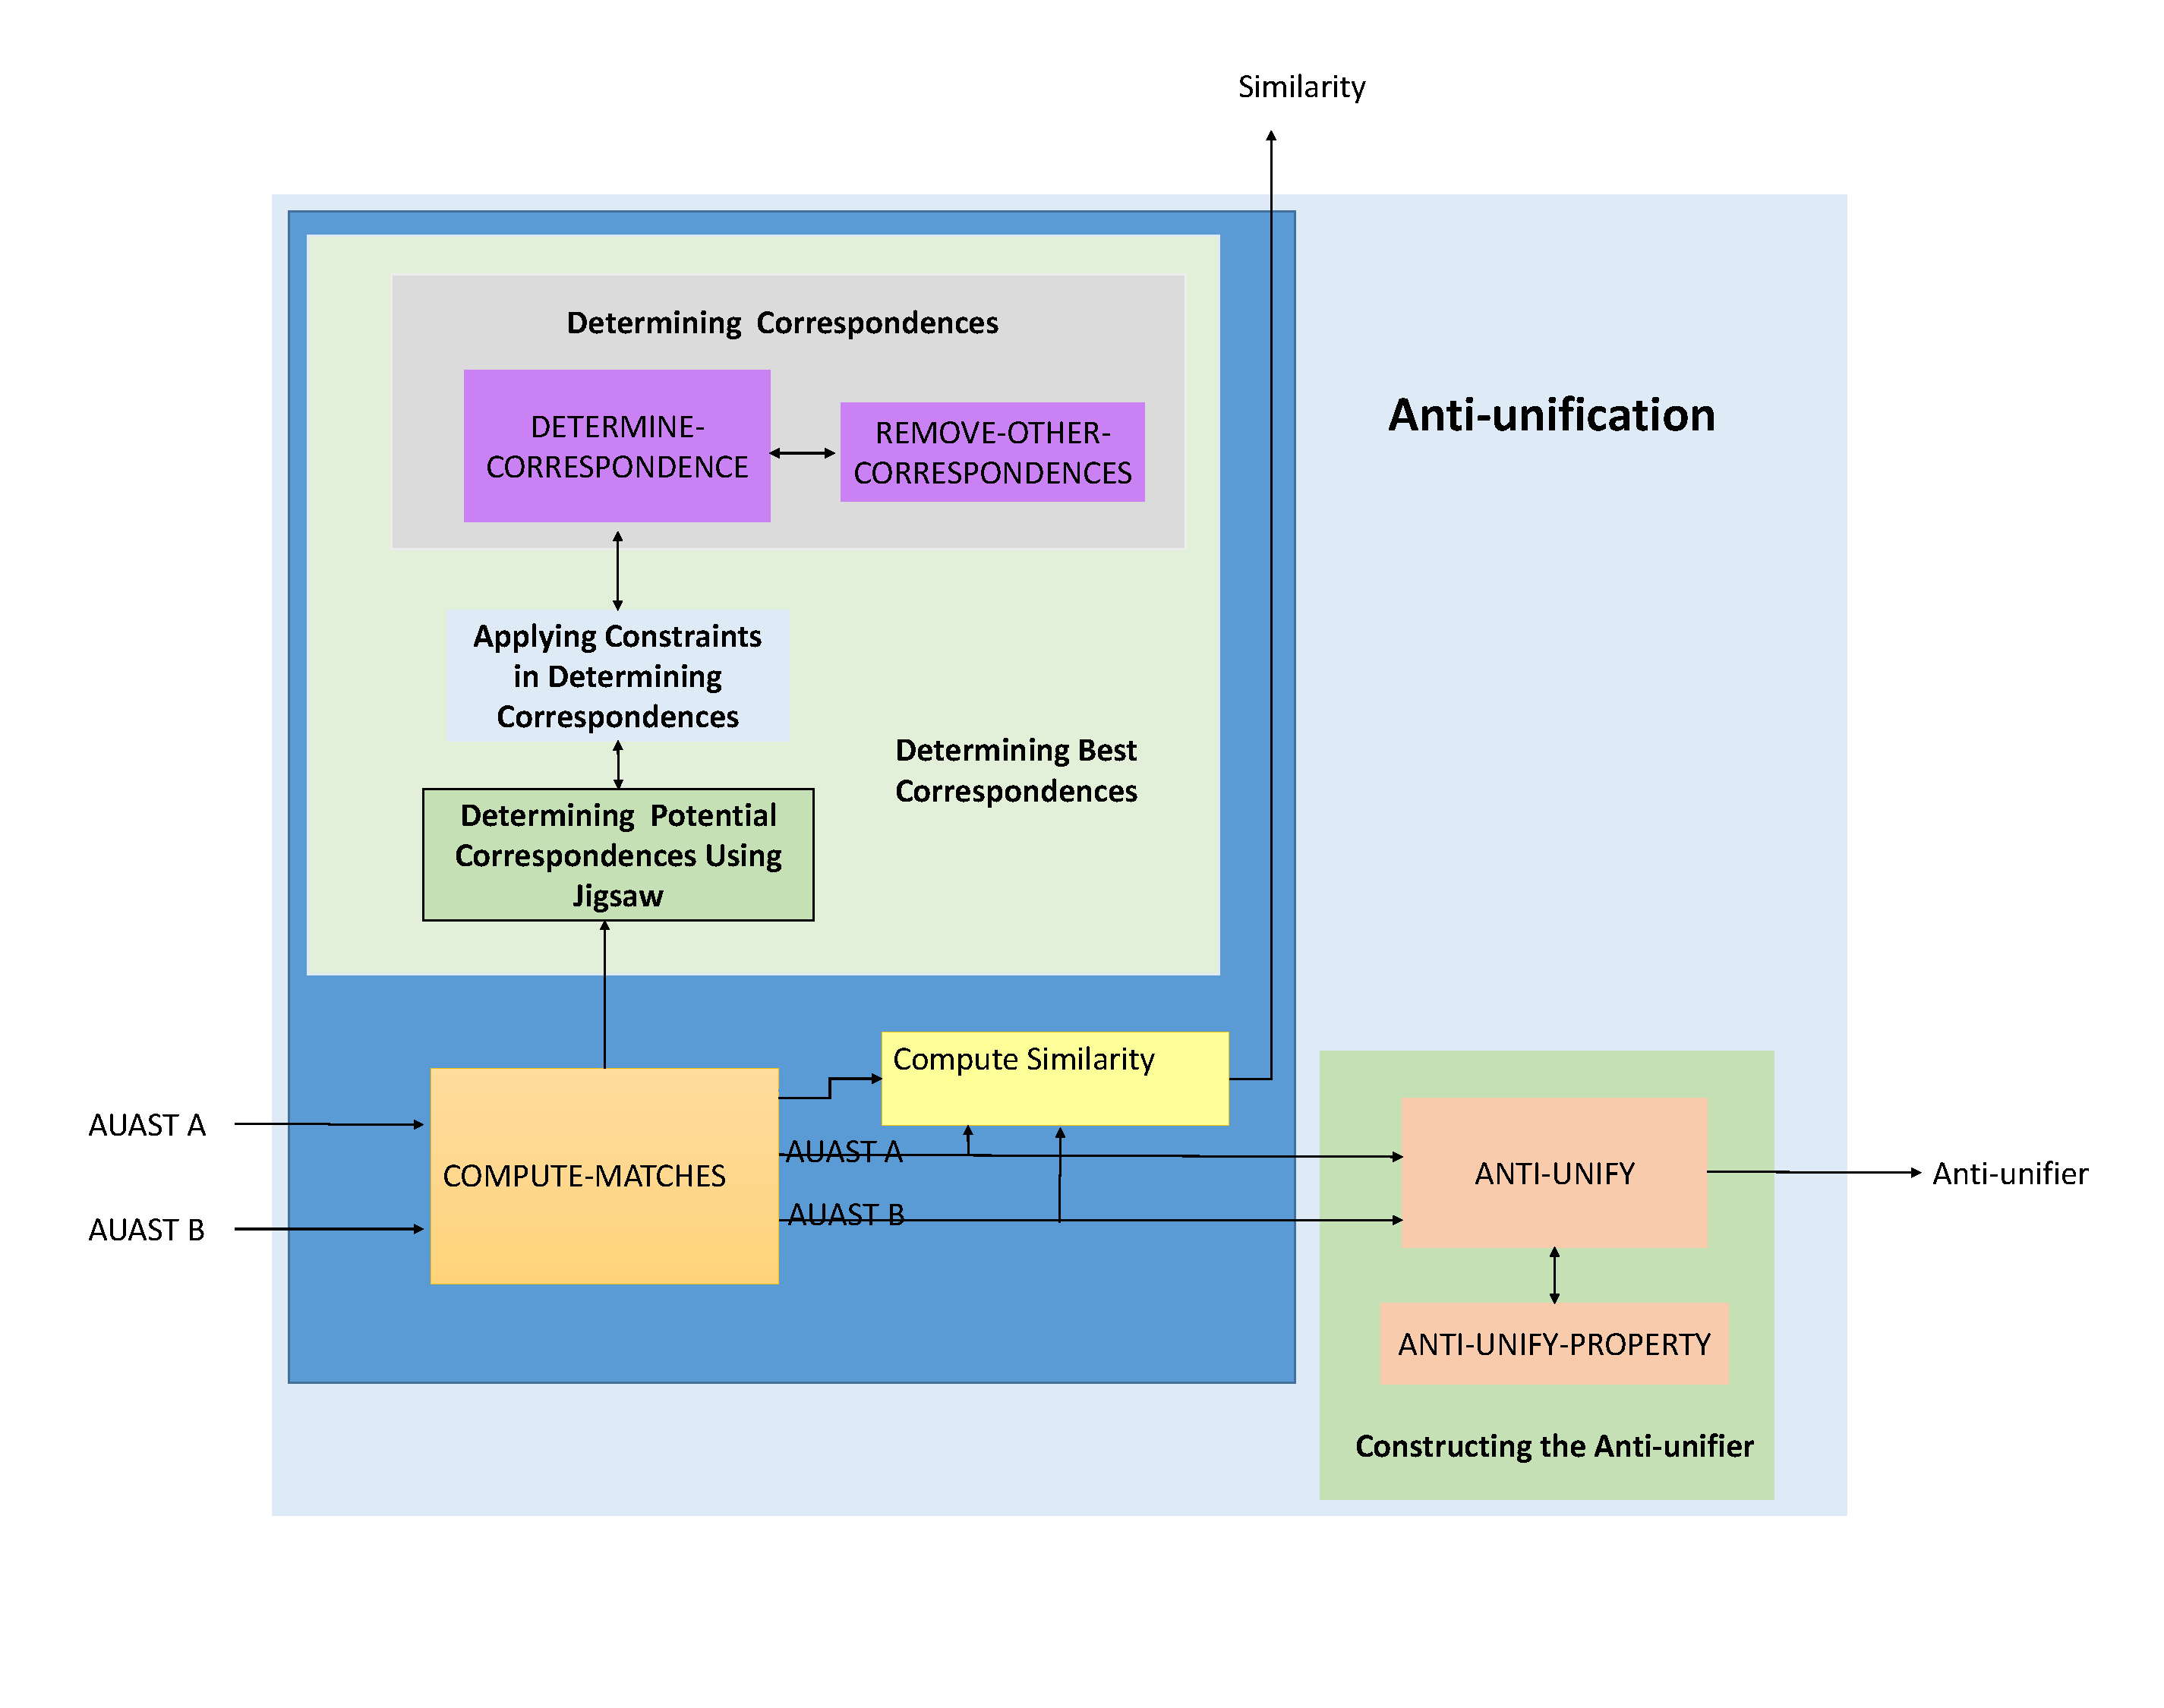
\includegraphics [width = \textwidth]{Drawing4/overview1.pdf}
  \caption{Overview of the anti-unification process.}
  \label{fig:meth_overview}
\end{figure}

To evaluate our anti-unification approach, we have developed the anti-unifier-building tool atop Jigsaw, and conducted an empirical study on a test suite. In Section~\ref{anti-unifier-assessment}, we describe our experimental setup, present our study, and discuss the results.  



%abstracts structural correspondences of ASTs

%A generalization mechanism could be used to abstract commonalities in several structures containing logging calls into a more general structure;
%The higher-order anti-unification modulo theories framework could assist us in constructing a structural generalization from a pair of LCSs. Also, A modified version of a hierarchical clustering suited for our application could assist us to construct a generalization from a set of LJMs.

%To construct a structural generalization from a pair of LJMs, we developed a prototype tool that applies the Jigsaw framework to find candidate correspondences between two ASTs and uses higher-order anti-unification modulo theories to generalize the structures. It takes the source code of two logged Java methods as input and performs a sequence of six actions on them, outlined by the algorithm \func{Anti-unification}: (1) we input into the algorithm the ASTs of two given logged Java methods, constructed via the Eclipse Java Development Tools (JDT) framework; (2) we generate an augmented form of AST (called a CAST) using the Jigsaw framework, where each node holds a list of candidate correspondence connections between the two ASTs (line~1) (see Section~\ref{meth-CAST}); (3) we extend the CAST structure to a higher-order extended structure (called an AUAST) and apply some constraints to prevent the anti-unification of logging calls with anything else (lines~2--3) (see Sections~\ref{meth-constructAUAST} and~\ref{meth-constraints}); (4) we determine the best correspondence for each node of the AUASTs with the highest similarity and we remove the other correspondence connections involving the nodes (line~4) (see Section~\ref{meth-correspondence}); (5) we anti-unify structural properties with their best correspondence to construct an approximation of the best anti-unifier to our problem with special attention to logging calls (line~5) (see Section~\ref{meth-antiUnifier}); and (6) we measure similarity (line~6) (see Section~\ref{meth-similarity}).
%\begin{algorithm}
%\caption{Input into \func{Anti-unification}(\id{auastA},\id{auastB}) are AUAST nodes of two Java classes containing logging calls; this algorithm construct an anti-unified AUAST node through anti-unification of input node's structural properties} %and compute similarity between them with a focus on logging calls}
%\label{overview}
%\begin{algorithmic}[1]
%\antiunification
%    \State  $\func{Jigsaw-Correspondence}(\id{auastA},\id{auastB})$
%   \State $\id{auastA}, \id{auastB} \gets \func{Apply-Constrains}(\id{auastA},\id{auastB})$
%   \State $$list}  \gets \func{Determine-Best-Correspondences}(\id{auastA})$
%     \State $$compute-similarity} \gets \func{Compute-Similarity}(\id{auastA},\id{auastB})$
%    \State $$anti-unifier} \gets \func{Antiunify}(\id{auastA},\id{auastB})$
%\end{algorithmic}
%\end{algorithm}


%\section{Anti-unification of a pair of ASTs} \label{anti-unification pairs} 
%\subsection{Anti-unification ASTs}\label{AUAST}
%\RW{Describe testing/evaluation.}


%\section{Anti-unification ASTs} \label{anti-unification pairs} 

\section{Constructing the AUAST} \label{AUAST}
\RW{This is a concrete implementation, not a generic idea, at least not the way it is described. I strongly suggest that you give a generic description of your assumptions about ASTs then relate AUASTs to those, then talk about implementation details.}
\NZ{I tried to explain it as an idea, does it make sense now?}
%An anti-unifier AST (AUAST) is an extended form of AST that allows the insertion of variables in place of any node in the tree structure, including both subtrees and leaves, to indicate variations between original structures. The AUAST addresses the limitations of AST to construct an anti-unifier by adding the following structural properties:


The goal of this phase is to construct an extended form of AST structure that would allow the creation of an anti-unified structure. As described in Section~\ref{HOAUMT}, an anti-unified structure utilizes variables that must be substituted with proper substructures to regain original structures. However, an AST structure does not contain any variables, and therefore an extended form of it is required, namely the AUAST (anti-unifier AST), that would allow the insertion of variables in place of any node in the tree structure, including both subtrees and leaves, to indicate variations between the original structures. The AUAST structure addresses the limitations of AST to construct an anti-unifier by adding the following structural properties:

\begin{itemize} [leftmargin=.5in]
\item \textit{Simple Variable Property}: an extension of simple property referring to two simple values to allow the insertion of variables in place of leaves.
\end{itemize}
\begin{itemize} [leftmargin=.5in]
\item \textit{Child Variable Property}: an extension of child property referring to two child AST nodes to allow the insertion of variables in place of subtrees.
\end{itemize}

To provide an example to demonstrate the AUAST, the anti-unified AUAST structure constructed from the AUASTs of logging calls in Figures~\ref{ch3-ex1} and~\ref{ch3-ex2} is depicted in Figure~\ref{fig:logging-anti}. The structural variables $X$ and $Y$ are used to indicate the structural variations, where the $X$ structural variable refers to two simple values and the $Y$ structural variable refers to two child nodes. The substitutions are defined in Equations~\ref{eq:theta1} and~\ref{eq:theta2}.

\begin{align}
\Theta_1 = (X \rightarrow \text{ \textsf{\small WARNING}}, Y \rightarrow \text{ \textit{additionExpression}(}\hspace*{3cm}\nonumber\\
\text{\textit{methodCall}(\textit{simpleName}(\textsf{\small getClassName}), \textit{arguments}()),}\nonumber\\
\text{\textit{stringLiteral}(\textsf{\small "should extend ..."}),}\hspace*{4cm}\nonumber\\
\text{\textit{methodCall}(\textit{simpleName}(\textsf{\small handleMessage}), \textit{arguments}()))})\hspace*{-1em}\label{eq:theta1}
\end{align}

\begin{align}
\Theta_2 = (X \rightarrow \text{ \textsf{\small ERROR}}, Y \rightarrow \text{ \textit{additionExpression}(}\hspace*{3cm}\nonumber\\
\text{\textit{stringLiteral}(\textsf{\small "Unknown action: "})},\nonumber\\
\text{ \textit{simpleName}(\textsf{\small actionName}))})\hspace*{-1cm}\label{eq:theta2}
\end{align}

%\item it can be mapped to our recursive definition of a term, where AST nodes and simple values may be viewed as function-symbols and constants, respectively

\begin{figure}[H]
\begin{small}
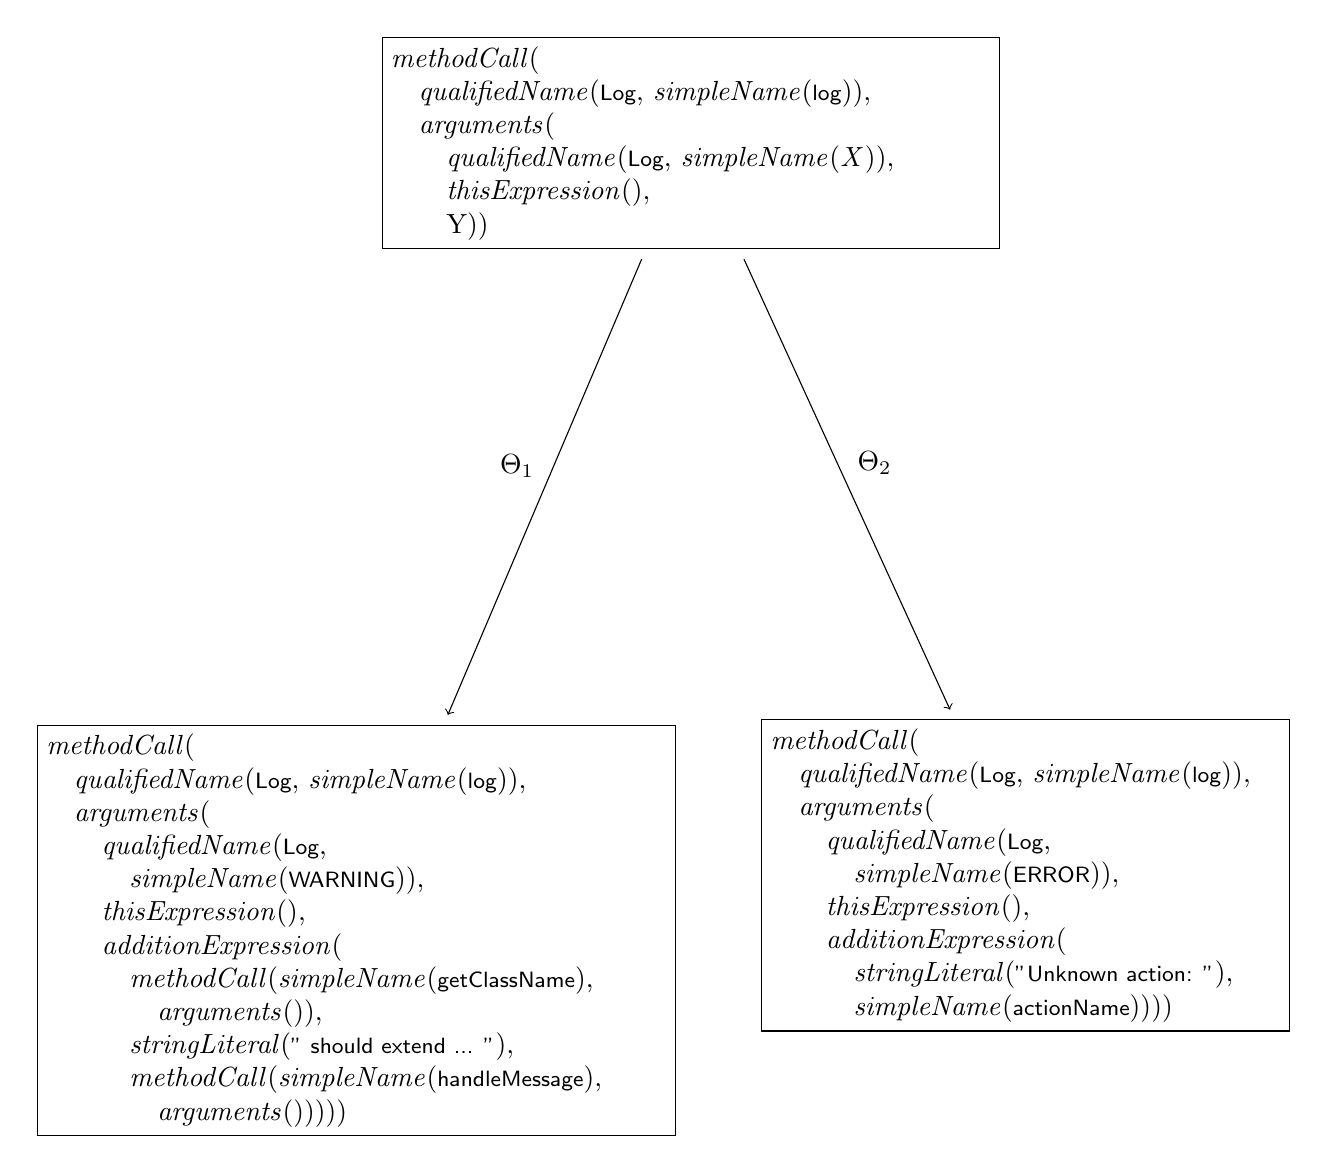
\begin{tikzpicture}
\node(a) at (4.25,10) {%
\fbox{\parbox[b][][b]{3in}{%
\text{\textit{methodCall}(}\\
\text{\hspace*{1em}\textit{qualifiedName}(\textsf{\footnotesize Log}, \textit{simpleName}(\textsf{\footnotesize log})),}\\
\text{\hspace*{1em}\textit{arguments}(}\\
\text{\hspace*{2em}\textit{qualifiedName}(\textsf{\footnotesize Log}, \textit{simpleName}(\textit{X})),}\\
\text{\hspace*{2em}\textit{thisExpression}(),}\\
\text{\hspace*{2em}Y))}}}%
};
\node(b) at (0,0) {%
\fbox{\parbox[t][][b]{3.1in}{%
\text{\textit{methodCall}(}\\
\text{\hspace*{1em}\textit{qualifiedName}(\textsf{\footnotesize Log}, \textit{simpleName}(\textsf{\footnotesize log})),}\\
\text{\hspace*{1em}\textit{arguments}(}\\
\text{\hspace*{2em}\textit{qualifiedName}(\textsf{\footnotesize Log},}\\ \text{\hspace*{3em}\mbox{\textit{simpleName}(\textsf{\footnotesize WARNING})}),}\\
\text{\hspace*{2em}\textit{thisExpression}(),}\\
\text{\hspace*{2em}\textit{additionExpression}(}\\
\text{\hspace*{3em}\textit{methodCall}(\textit{simpleName}(\textsf{\footnotesize getClassName}),}\\ \text{\hspace*{4em}\textit{arguments}()),}\\
\text{\hspace*{3em}\textit{stringLiteral}(\textsf{\footnotesize " should extend ... "}),}\\
\text{\hspace*{3em}\textit{methodCall}(\textit{simpleName}(\textsf{\footnotesize handleMessage}),}\\ \text{\hspace*{4em}\textit{arguments}()))))}}}%
};
\node(c) at (8.5,0.7) {%
\fbox{\parbox[t][][b]{2.55in}{%
\text{\textit{methodCall}(}\\
\text{\hspace*{1em}\textit{qualifiedName}(\textsf{\footnotesize Log}, \textit{simpleName}(\textsf{\footnotesize log})),}\\
\text{\hspace*{1em}\textit{arguments}(}\\
\text{\hspace*{2em}\textit{qualifiedName}(\textsf{\footnotesize Log},}\\ \text{\hspace*{3em}\mbox{\textit{simpleName}(\textsf{\footnotesize ERROR})}),}\\
\text{\hspace*{2em}\textit{thisExpression}(),}\\
\text{\hspace*{2em}\textit{additionExpression}(}\\
\text{\hspace*{3em}\textit{stringLiteral}(\textsf{\footnotesize "Unknown action: "}),}\\
\text{\hspace*{3em}\textit{simpleName}(\textsf{\footnotesize actionName}))))}}}%
};

\draw[->](a) -- (b) node[pos=0.5,above]{$\Theta_1\qquad$};
\draw[->](a) -- (c) node[pos=0.5,above]{$\qquad\Theta_2$};
\end{tikzpicture}
\end{small}
\caption{Anti-unification of the AUASTs of the logging calls in Examples 1 and 2.\label{fig:logging-anti}}
\end{figure}
%The AUASTs of log Method Invocation nodes from the Java classes in Figure~\ref{ch3-ex1} and Figure~\ref{ch3-ex2}.




%\begin{align}
%\Theta_1 = (W &\rightarrow \text{ \textsf{\small WARNING}},\nonumber\\
%X &\rightarrow \text{ \textit{methodCall}(\textit{simpleName}(\textsf{\small getClassName}), \textit{arguments}())},\nonumber\\
%Y &\rightarrow \text{ \textsf{\small "should extend EditPlugin not EBPlugin since it has an empty "}},\nonumber\\
%Z &\rightarrow \text{ \textit{methodCall}(\textit{simpleName}(\textsf{\small handleMessage}), \textit{arguments}())})\label{eq:theta1}\\
%\Theta_2 = (W &\rightarrow \text{ \textsf{\small ERROR}},\nonumber\\
%X &\rightarrow \text{ \NIL{}},\nonumber\\
%Y &\rightarrow \text{ \textsf{\small "Unknown action: "}},\nonumber\\
%Z &\rightarrow \text{ \textit{simpleName}(\textsf{\small actionName})})\label{eq:theta2}
%\end{align}
%
%%\item it can be mapped to our recursive definition of a term, where AST nodes and simple values may be viewed as function-symbols and constants, respectively
%
%\begin{figure}[p]
%\begin{small}
%\begin{tikzpicture}
%\node(a) at (4.25,10) {%
%\fbox{\parbox[b][][b]{3in}{%
%\text{\textit{methodCall}(}\\
%\text{\hspace*{1em}\textit{qualifiedName}(\textsf{\footnotesize Log}, \textit{simpleName}(\textsf{\footnotesize log})),}\\
%\text{\hspace*{1em}\textit{arguments}(}\\
%\text{\hspace*{2em}\textit{qualifiedName}(\textsf{\footnotesize Log}, \textit{simpleName}(\textit{W})),}\\
%\text{\hspace*{2em}\textit{thisExpression}(),}\\
%\text{\hspace*{2em}\textit{additionExpression}(\textit{X}, \textit{stringLiteral}(\textit{Y}), \textit{Z})))}}}%
%};
%\node(b) at (0,0) {%
%\fbox{\parbox[t][][b]{3.1in}{%
%\text{\textit{methodCall}(}\\
%\text{\hspace*{1em}\textit{qualifiedName}(\textsf{\footnotesize Log}, \textit{simpleName}(\textsf{\footnotesize log})),}\\
%\text{\hspace*{1em}\textit{arguments}(}\\
%\text{\hspace*{2em}\textit{qualifiedName}(\textsf{\footnotesize Log},}\\ \text{\hspace*{3em}\mbox{\textit{simpleName}(\textsf{\footnotesize WARNING})}),}\\
%\text{\hspace*{2em}\textit{thisExpression}(),}\\
%\text{\hspace*{2em}\textit{additionExpression}(}\\
%\text{\hspace*{3em}\textit{methodCall}(\textit{simpleName}(\textsf{\footnotesize getClassName}),}\\ \text{\hspace*{4em}\textit{arguments}()),}\\
%\text{\hspace*{3em}\textit{stringLiteral}(\textsf{\footnotesize " should extend ... "}),}\\
%\text{\hspace*{3em}\textit{methodCall}(\textit{simpleName}(\textsf{\footnotesize handleMessage}),}\\ \text{\hspace*{4em}\textit{arguments}()))))}}}%
%};
%\node(c) at (8.5,0.7) {%
%\fbox{\parbox[t][][b]{2.55in}{%
%\text{\textit{methodCall}(}\\
%\text{\hspace*{1em}\textit{qualifiedName}(\textsf{\footnotesize Log}, \textit{simpleName}(\textsf{\footnotesize log})),}\\
%\text{\hspace*{1em}\textit{arguments}(}\\
%\text{\hspace*{2em}\textit{qualifiedName}(\textsf{\footnotesize Log},}\\ \text{\hspace*{3em}\mbox{\textit{simpleName}(\textsf{\footnotesize ERROR})}),}\\
%\text{\hspace*{2em}\textit{thisExpression}(),}\\
%\text{\hspace*{2em}\textit{additionExpression}(}\\
%\text{\hspace*{3em}\textit{stringLiteral}(\textsf{\footnotesize "Unknown action: "}),}\\
%\text{\hspace*{3em}\textit{simpleName}(\textsf{\footnotesize actionName}))))}}}%
%};
%
%\draw[->](a) -- (b) node[pos=0.5,above]{$\Theta_1\qquad$};
%\draw[->](a) -- (c) node[pos=0.5,above]{$\qquad\Theta_2$};
%\end{tikzpicture}
%\end{small}
%\caption{The anti-unification of the AUASTs of the logging calls in Examples 1 and 2.\label{fig:logging-anti}}
%\end{figure}
%%The AUASTs of log Method Invocation nodes from the Java classes in Figure~\ref{ch3-ex1} and Figure~\ref{ch3-ex2}.

%Applying higher-order anti-unification on AUAST structures could help to construct a structural generalization by maintaining the common pieces and abstracting the differences away using variables. However, it is not comprehensive enough to solve our problem as it does not consider background knowledge about AST structures, such as syntactically different but semantically relevant structures, missing structures, and different ordering of arguments. In the following section, we will look at an extension of anti-unification, higher-order anti-unification modulo theories, and how it can sufficiently address the limitations of anti-unification in our context.

%We provide an example to demonstrate the AUAST structure, which is limited to log method invocation subtrees of the sample Java classes shown in Figure~\ref{fig:constructAUast}. The log method invocation nodes both contains \texttt{EXPRESSION}, \texttt{ARGUEMENTS}, and \texttt{NAME} structural properties which are made up of \texttt{\bold{Log}}, \texttt{\bold{Log}}, \texttt{\bold{WARNING}} simple values for the AUAST1 and  \texttt{\bold{Log}}, \texttt{\bold{Log}}, \texttt{\bold{ERROR}} simple values for the AUAST2, respectively. The structural representation of the AUASTs as defined in Section~\ref{back-str} is \texttt{EXPRESSION[EXPRESSION[IDENTIFIER[\bold{Log}]], ARGUMENTS[QUALIFIER[IDENT\\IFIER[\bold{Log}]], NAME[IDENTIFIER[\bold{WARNING}]]}for the AUAST1 and \texttt{EXPRESSION[EX\\PRESSION[IDENTIFIER[\bold{Log}]], ARGUMENTS[QUALIFIER[IDENTIFIER[\bold{Log}]], \\NAME[IDENTIFIER[\bold{ERROR}]]} for the AUAST2, where the words capitalized represents subtrees and the words shown in bold represents leaves of the tree structure.

%\begin{figure} [H]
 % \centering\includegraphics [width = \textwidth, height = 0.4\textheight]
 % {Drawing4/structure1.pdf}
 % \caption{The AUASTs of log Method Invocation nodes from the Java classes in Figure~\ref{ch3-ex1} and Figure~\ref{ch3-ex2}.}
 % \label{fig:constructAUast}
%\end{figure}


\section{Determining potential correspondences using the Jigsaw framework} \label{meth-CAST}
To construct the best anti-unifier from two given AUASTs using an approximation technique, we should first determine candidate structural correspondences between AUAST nodes and then select the best candidate with the highest similarity for each node. The Jigsaw framework can help to detect candidate correspondences and measure similarity between the nodes involved in each correspondence, as described in Chapter~\ref{background2}. 

%\begin{algorithm}
%\caption{\func{Jigsaw-Correspondence}($\id{auastA}$, $\id{auastB}$) determines potential correspondences between nodes of two given AUASTs}
%\label{overview}
%\begin{algorithmic}[1]
%\JigsawCorr
%\For $\id{astA} \in  \id{auastA}$
%\For $\id{astB} \in  \id{auastB}$		
%	\State  $\id{castA},\id{castB} \gets \func{Jigsaw-Antiunify}(\id{astA},\id{astB})$
%\EndFor	
%\EndFor
%\end{algorithmic}
%\end{algorithm}

\section{Constraints in Determining Correspondences}  \label{meth-constraints}
To construct an anti-unifier of two AUASTs with a focus on logging calls, some constraints should be applied prior to determining the best correspondences. The first constraint (as described below) should be applied to prevent the anti-unification of log method invocation nodes with any other type of node.
\begin{constraint}
A logging call should either be anti-unified with another logging call or should be anti-unified with \nothing.
\end{constraint}	
	
This constraint creates a further constraint:

\begin{constraint}
A structure containing a logging call should be anti-unified with a corresponding structure containing another logging call or should be anti-unified with \nothing.
\end{constraint}

As an illustration consider AUASTs of two Java classes in Figure~\ref{fig:meth-ast-1}. Jigsaw creates a correspondence connection between the two log method invocation nodes and the two \code{if} statements. As is clear, the second \code{if} statement contains a logging call, while there is no corresponding logging call in the first one. According to the first constraint, two log method invocation nodes should be anti-unified together. On the other hand, a correspondence connection is created between the two \code{if} statements; however, anti-unification of these statements includes anti-unifying their children nodes as well. Thus, statements inside the body of the \code{if} statements must be anti-unified with each other, indicating that log method invocation inside the body of \code{if} statement in the second example should be anti-unified with \nothing, which is contrary to our first assumption. In order to comply with the first constraint, the correspondence connection between two \code{if} statements should be deleted, leading us to apply the second constraint.

Our approach applies these constraints by taking the following steps prior to determining the best correspondences:
\begin{enumerate} [leftmargin=.4in]
\item	Augment a property to the AUAST node to mark log method invocation nodes and structures enclosing them as ``logged''.

\item	Remove correspondence connections where one node is marked as ``logged'' and the corresponding node is not.
\end{enumerate}


\section{Determining Correspondences} \label{meth-correspondence}
As described in Section~\ref{Jigsaw}, through the application of the Jigsaw framework, each AUAST node will hold a list of candidate correspondence connections, each implicitly representing an anti-unifier. However, despite having multiple potential anti-unifiers, we need to determine one single anti-unifier that is helpful to solve our problem. To do so, we have developed \func{Determine-Correspondence} algorithm that greedily selects the most similar correspondence as the best fit for each AUAST node. Therefore, each AUAST node can either be anti-unified with its best correspondence in the other AUAST or with \nothing in a later step. This algorithm should be used after applying the constraints mentioned in Section~\ref{meth-constraints} on candidate correspondence connections. 

%In general, higher order anti-unification modulo theories is undecidable [Cottrell et al., 2008]. That is, the complexity of determining the most optimal MSA is undecidable, but our desire is to create one of the best MSAs to approximate the optimal one that can sufficiently solve our problem, thus the anti-unification process should construct an anti-unifier that is the best approximate fit for our application. To this end, a greedy selection algorithm has been used, which is an approximation technique to determine the best correspondence for each node in the AUAST so constructing the anti-unifier that is approximately the best fit to our problem.

The \func{Determine-Correspondence} algorithm takes one of the AUASTs, visiting the AUAST nodes therein to store all candidate correspondence connections between the two AUAST nodes in a list, which is sorted in descending order based on the Jigsaw similarity measure (lines~1--8). The correspondence connection with the highest similarity value is determined as the best fit for the two nodes involved (lines~9--11); all other correspondence connections involving these two nodes are removed using \func{Remove-Other-Correspondences} algorithm (line~10). This process terminates when no more correspondence connections are left in the list.
\begin{algorithm}
\caption{\func{Determine-Correspondence}($\id{auastA}$) takes in an AUAST and determines the best correspondence connection with the highest similarity for each AUAST node.}
\label{alg-determine}
\begin{algorithmic}[1]
\CreateList
    \State $\id{list} \gets \func{()}$
    \State $\id{nodes} \gets \func{visitor}(\id{auastA})$
	  \For {$\id{node} \in \id{nodes}$}
	
				\For {$\id{ce} \in  \id{correspondences}[\id{node}]$}		
				 	\State{$\func{Append}(\id{ce},\id{list})$ }
			 	\EndFor  	
	   \EndFor		
	   \State{$\func{sort}(\id{list})$}
	   \For{$\id{ce} \in \id{list}$}
	   		\State{$\func{Remove-Other-Correspondences}(\id{ce},\id{list})$ }
	   \EndFor
 %\Return $\id{list} $  	
  \end{algorithmic}
\end{algorithm}

\func{Remove-Other-Correspondences} algorithm removes correspondence connections that are not selected as the best fit from three lists: the list of all correspondence connections (Line~5 and Line~12);
the list of correspondence connections of the first node involved in the connection (Line~6 and Line~13); the list of correspondence connections of the second node involved in the connection (Line~7 and Line~14).

\begin{algorithm}
\caption{\func{Remove-Other-Correspondences}($\id{ce}$, $\id{list}$) removes all other correspondences involving nodes of a particular correspondence connection or element ($\id{ce}$) from the lists of correspondence connections.}
\label{removeOtherCEs}
  \begin{algorithmic}[1]
  \RemoveOtherCEs
       \State $\id{list1} \gets \id{correspondences}[\id{nodeA}[\id{ce}]]$
	   \State $\id{list2} \gets \id{correspondences}[\id{nodeB}[\id{ce}]]$
	   \For {$\id{ce1} \in \id{list1}$}
			\If{$\id{ce1} \neq \id{ce}$}	
\State{$\func{Remove}(\id{ce1},\id{list})$ } 			
\State{$\func{Remove}(\id{ce1},\id{correspondences}[\id{nodeA}[\id{ce1}]])$ }
\State{$\func{Remove}(\id{ce1},\id{correspondences}[\id{nodeB}[\id{ce1}]])$ }    		
	   		 \EndIf
	   \EndFor		
       \For {$\id{ce2} \in \id{list2}$}
			\If{$\id{ce2} \neq \id{ce}$}	   		 	 	
	 	 	\State{$\func{Remove}(\id{ce2},\id{list})$ } 		 \State{$\func{Remove}(\id{ce2},\id{correspondences}[\id{nodeA}[\id{ce2}]])$ }
\State{$\func{Remove}(\id{ce2},\id{correspondences}[\id{nodeB}[\id{ce2}]])$ }
	   		 \EndIf
	   \EndFor	  	
  \end{algorithmic}
\end{algorithm}

As an example, Figure~\ref{fig:AUASTs} shows the correspondences between AUAST nodes after applying the constraints and the \func{Determine-Correspondence} algorithm on the list of potential correspondence connections created by the Jigsaw framework in Figure~\ref{fig:meth-ast-1}.
%EXPLAIN MORE ?

\begin{figure} [H]
  \centering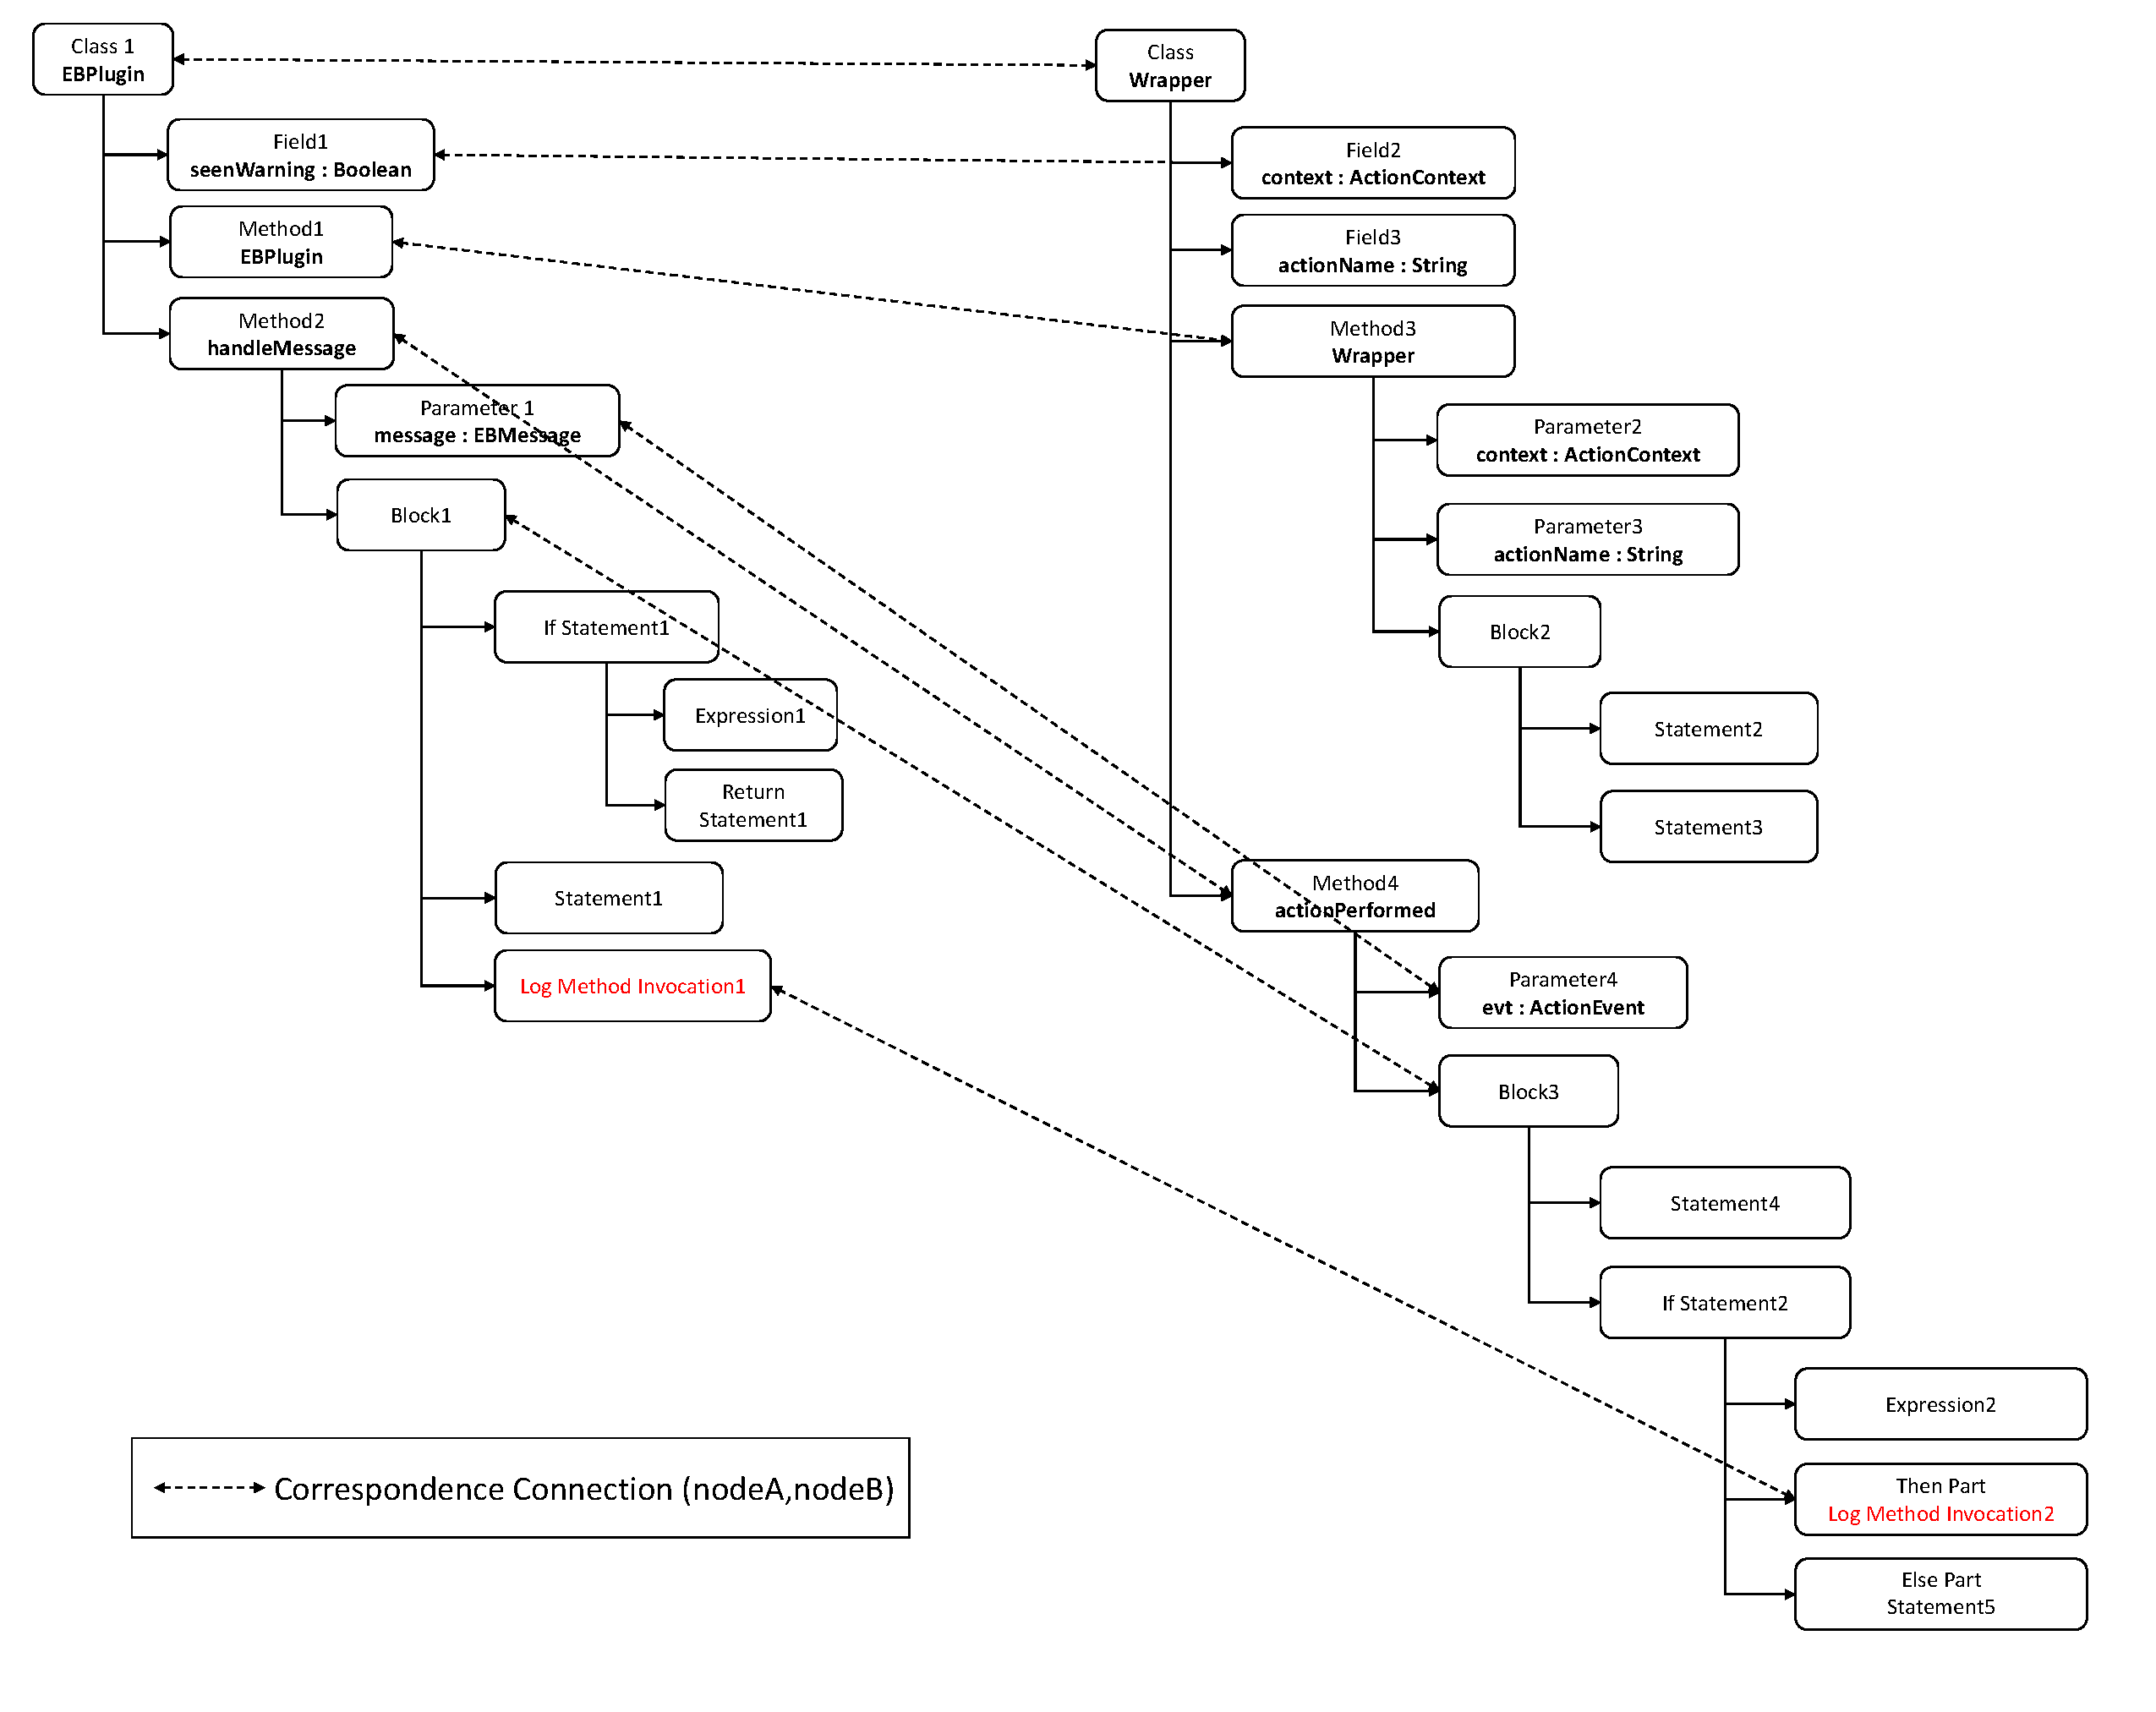
\includegraphics [width = \textwidth]{Drawing4/FinalCorr.pdf}
  \caption{Simple AUAST structure of examples in Figures~\ref{ch3-ex1} and~\ref{ch3-ex2}. The links between AUAST nodes indicate structural correspondences selected as the best fit by the \func{Determine-Correspondence} algorithm.}
  \label{fig:AUASTs}
\end{figure}


\section{Constructing the anti-unifier} \label{meth-antiUnifier}
Once the best correspondences have been determined between AUAST nodes, we construct a new anti-unified AUAST by traversing AUAST structures recursively and anti-unifying the structural properties. The new anti-unified structure is a generalization of two original structures, called anti-unifier, where common structural properties are represented by copies and differences are represented by structural variables. The variables may be inserted in place of any node in AUAST, including both subtrees and leaves, and can be substituted with proper original substructures to regain original structures.

Anti-unification of two AUASTs is performed through the anti-unification of their structural properties, via the \func{Antiunify} algorithm. For each structural property of $\id{auastA}$ and $\id{auastB}$, where there is no corresponding property in the other AUAST, a structural variable property is created by anti-unifying the structural property with the \NIL{} structure via the \func{Antiunify-Property} algorithm and is added to properties of the anti-unifier (Lines~4-5 and Lines~13-15); if both nodes have the same property but with different property values, a structural variable property is created via the \func{Antiunify-Property} algorithm and appended to the anti-unifier structural properties (Lines~6-7); otherwise, if the two nodes have the same exact structural property, a copy of one of them is added to the anti-unifier structural properties (Lines~8-9).


\begin{algorithm}
 \caption{Inputs into \func{Antiunify}($\id{auastA}$, $\id{auastB}$) are two AUASTs. This algorithm construct an anti-unified AUAST through the anti-unification of input nodes' structural properties.}
  \label{AntiUnify}
  \begin{algorithmic}[1]
\AntiUnify
\State{$ \id{antiunifier} \gets \cons{Null}$}
\For {$\id{propA} \in \id{properties}[\id{auastA}]$}
	\State{$ \id{valueA} \gets \id{value}[\id{property}]$}
	\If {$ \func{contains}(\id{auastB},\id{propA})= \cons{NULL}$}
		\State{$\func{AddProperty}(\id{antiunifier}, \func{Antiunify-Property}(\id{propA},\cons{NIL}))$}
	\ElsIf{$ \id{valueA} \neq \id{value}[\func{contains}(\id{auastB},\id{propA})]$}
	\State{$\func{AddProperty}(\id{antiunifier}, \func{Antiunify-Property}(\id{propA},\func{contains}(\id{auastB},\id{propA}))$}
	\Else
     \State{$\func{AddProperty}(\id{antiunifier}, \id{propA})$}
	\EndIf
\EndFor
\For {$\id{propB} \in \id{properties}[\id{auastB}]$}
	\If {$ \func{contains}(\id{auastA},\id{propB})= \cons{NULL}$}
		\State{$\func{AddProperty}(\id{antiunifier}, \func{Antiunify-Property}(\id{propB},\cons{NIL}))$}
	
	\EndIf	
\EndFor
\Return $\id{antiunifier}$
\end{algorithmic}
\end{algorithm}

Anti-unification of structural properties $\id{propA}$ and $\id{propB}$ is performed via the \func{Antiunify-Property} algorithm. If $\id{propA}$ is a simple property, a simple variable property is constructed referring to two simple values (Lines~2-3); if structural property is a child property, a child variable structure is constructed (Line~5); if structural property is a child list property, for each child of $\id{propA}$ and $\id{propB}$, where there is no correspondence in the other AUAST, an anti-unified node is created through anti-unifying the child node with the \NIL{} structure via the \func{Antiunify} algorithm and added to the value of the anti-unified child list property; otherwise, the child node is anti-unified with its best correspondence (Lines~6-20).


\begin{algorithm}
 \caption{\func{Antiunify-Property}($\id{propA}$, $\id{propB}$) takes two structural properties and constructs an anti-unified structural property.}
  \label{AntiUnify}
  \begin{algorithmic}[1]
\AntiUnifyProperty
\State{$ \id{property} \gets \cons{Null}$}

\If {$\id{propA}$  \Instanceof $\cons{SimpleProperty}$}
	      \State $\id{property} \gets  \func{Create-Simple-Variable-Property}(\id{propA},\id{propB})$
 	 \ElsIf {$\id{propA}$ \Instanceof $\cons{ChildProperty}$}
			\State $\id{property} \gets  \func{Create-Child-Variable-Property}(\id{propA},\id{propB})$
			 \ElsIf {$\id{propA}$ \Instanceof $\cons{ChildListProperty}$}
	
	\For {$\id{child} \in \id{value}[\id{propA}]$}	
	  \If {$\id{correspondence}[\id{child}] \neq \cons{NULL}$} 	
	  \State $\func{append}(\id{children},\func{Antiunify}(\id{child}, \id{correspondence}[\id{child}]))$
	   \Else 	
	    \State $\func{append}(\id{children},\func{Antiunify}(\id{child}, \cons{NIL}))$
	    \EndIf
      \EndFor
      \For {$\id{child} \in \id{value}[\id{propB}]$}	
	  \If {$\id{correspondence}[\id{child}] = \cons{NULL}$} 	          	
	    \State $\func{append}(\id{children},\func{Antiunify}(\id{child}, \cons{NIL}))$
	    \EndIf
      \EndFor
		%\State $ \id{value}[\id{property}] \gets\id{children} $
		\State $\id{property} \gets  \func{Create-Child-List-Property}(\id{children},\id{id[propA]})$
    \EndIf
\Return $\id{property}$
\end{algorithmic}
\end{algorithm}


For example, we supply the \func{Antiunify} algorithm with the AUASTs of LJMs in Examples 1 and 2. Figure~\ref{fig:meth-anti-unifier} shows a simple detailed view we used to represent the anti-unifier constructed from the two AUASTs, where ``$\id{a}$-or-$\id{b}$'' represents a structural variable that must be substituted with either $a$ or $b$ substructures to recover each original structure, and ``$\id{a}$'' represents that $a$  substructure is common between the two AUASTs.


\begin{figure} [H]
  \centering\includegraphics [width = 0.8\textwidth, height = 0.9\textheight]{Drawing4/anti-unifier.pdf}
  \caption{Simple detailed view of the anti-unifier constructed from the AUASTs of the LJMs in Example s 1 and 2.}
  \label{fig:meth-anti-unifier}
\end{figure}




%For example, we supply \func{Antiunify} algorithm with the log method invocation nodes from the AUASTs in Figure~\ref{fig:constructAUast}. \texttt{EXPRESSION} and \texttt{ARGUMENTS} are similar in both AUASTs thus a copy of them will be added to structural properties of the anti-unified AUAST (Line~10); however, the simple value of Name property is different in both structures thus a call to \func{Antiunify-Property} on Line~8 will return a simple structural variable. Figure~\ref{fig:AUAUAST} shows the anti-unified AUAST, where the annotation \texttt{WARNING-or-ERROR} is used to represent the simple structural variable that must be substituted with either \texttt{WARNING} or \texttt{ERROR} simple value to gain back to each original AUAST structure. The structural representation of the anti-unified AUAST is \texttt{EXPRESSION[EXPRESSION[IDENTIFIER[\bold{Log}]], ARGUMENTS[QUALIFIER[IDENTI\\FIER[\bold{Log}]], NAME[IDENTIFIER[\bold{WARNING-or-ERROR}]]}.

%\begin{figure} [H]
 % \centering\includegraphics [width = 0.5\textwidth, height = 0.35\textheight]
  %{Drawing4/structureAU.pdf}
  %\caption{The anti-unifier (AUAST3) constructed from log Method Invocation AUAST nodes in Figure~\ref{fig:constructAUast} }
  %\label{fig:AUAUAST}
%\end{figure}

%Figure~\ref{fig:meth-anti-unifier} shows a simple view of the anti-unified AUAST constructed from the two AUASTs in Figure~\ref{fig:AUASTs}, where ``$\id{a}\langle\rangle\id{b}$'' represents that the two subtrees $a$ and $b$ are anti-unified with each other in the anti-unifier and ``$\id{a}$-or-$\id{b}$'' represents a simple structural variable that must be substituted with either $a$ or $b$ simple value to recover each original structure.


%\begin{figure} [H]
%  \centering\includegraphics [width = 0.8\textwidth, height = 0.9\textheight]{Drawing4/anti-unifier.pdf}
 % \caption{Simple anti-unified AUAST structure of the two  AUASTs in Figure~\ref{fig:AUASTs}}
  %\label{fig:meth-anti-unifier}
%\end{figure}


\section{Computing Similarity} \label{meth-similarity}
Similarity computation is particularly important for clustering phase that relies on accurate estimation of similarity between logged Java methods and will be discussed in detail in Section~\ref{clustering}. The notion of similarity can differ depending on the given context. That is, similarity between certain features could be highly important for a particular application, while it is not for another. The utility of a similarity function can be determined based on how well it enables us to produce accurate results for a particular task. In this study, a similarity measure is needed to classify Java methods that use logging calls based on the structural similarity between them. The structural similarity of two AUASTs can be defined as the number of identical simple structural property values over the total number of simple structural property values of the anti-unifier.

\begin{algorithm}
  \caption{\func{Compute-Matches}($\id{auastA}$) takes in one of the AUASTs and determines the matches between the two AUASTs via a recursive traversal of structural properties.}
  \label{computeMatches}
  \begin{algorithmic}[1]
  \ComputeMatch
  	%\If {$\id{auastB} \neq \cons{NULL}$}
  	 %  \State{$ \func{Determine-Best-Correspondence}(\id{auastA}, \id{auastB})$}
  	  % \EndIf
         \State $\id{matches} \gets 0$
       \For {$\id{property} \in \id{properties}[\id{auastA}]$}
	\State $\id{valueA} \gets \id{value}[\id{property}]$
	\State $\id{valueB} \gets \func{Get-Best-Correspondence}(\id{valueA})$
       	\If {$\id{property}$  \Instanceof $\cons{SimpleProperty}$ }
 \State $\id{matches} \gets  \id{matches} + \func{Jigsaw-Matches}(\id{valueA}, \id{valueB})$ 	
	
 		\ElsIf {$\id{property}$ \Instanceof $\cons{ChildProperty}$ }		
	          \State $\id{matches} \gets  \id{matches} +\func{Compute-Matches}(\id{valueA})$		
	    \ElsIf {$\id{property}$ \Instanceof $\cons{ChildListProperty}$}
	\For {$\id{nodeA} \in \id{valueA}$}	
		\State $\id{nodeB} \gets \func{Get-Best-Correspondence}(\id{nodeA})$
	 \State $\id{matches} \gets  \id{matches} + \func{Compute-Matches}(\id{nodeA})$
	  \EndFor 	
	   \EndIf
       \EndFor 	
	\Return $\id{matches}$
  \end{algorithmic}
\end{algorithm}

%The number of matches
%reusing the Jigsaw???
The number of identical simple structural property values between $\id{auastA}$ and $\id{auastB}$ is computed via the \textsc{Compute-Matches} algorithm through a recursive traversal of $\id{auastA}$ nodes' structural properties. For simple structural properties, the number of matches is computed re-using the Jigsaw similarity function that computes the number of matches between the property values (Lines~5-6). For child structural properties, the number of matches is computed recursively for a child node and is propagated to the parent(Lines~7-8). For child list structural properties, the number of matches is computed for each child node recursively and is propagated to the parent node (Lines~9-14). All matches are summed up to compute total number of matches between the two AUASTs. Then the following equation is used to compute structural similarity between $\id{auastA}$ and $\id{auastB}$:
%First, the best correspondences are selected using the \func{Determine-Best-Correspondence} algorithm.
%get-best-correspondence input

\begin{equation}\label{eq1}
\id{similarity} = \frac{2*\id{matches}}{|\id{auastA}| + |\id{auastB}|}
\end{equation}

%Where total number of simple values for $\id{auastA}$ and $\id{auastB}$ is computed via \func{Compute-Matches}($\id{auastA}$) and \func{Compute-Matches}($\id{auastB}$), respectively.
The similarity function returns a value between 0 and 1 that indicates zero and total matching, respectively.

%The recursion process terminates if a simple or a variable structural property is reached.

\section{Multiple logging calls} \label{meth-multipleLogs}
There might be some cases in which our approach is not able to anti-unify logging calls in two input seeds, when there is more than one logging call in a logged Java method. For example, consider the logged Java methods in Figures~\ref{multiple1} and~\ref{multiple2}. Figure~\ref{mast_1} shows the simple AUASTs for these examples and potential correspondence connections between AUAST nodes. Figure~\ref{m_ast2} shows the correspondence connections selected as the best match using our greedy algorithm. To anti-unify \code{if statement 1} with \code{if statement 3}, we should anti-unify their structural properties. Thus, \code{log1} should be anti-unified with \code{log3} and \code{log4} should be anti-unified with \nothing{} since there is no corresponding logging call in the body of \code{if statement 1}, while there is a corresponding logging call for \code{log4} in the body of \code{if statement 2} (\code{log2}).


\begin{figure}[H]
\def\baselinestretch{1}
\begin{lstlisting}
public void method1(){
	...
	if(condition1){
		Log.log();
	}
	...
	if(condition2){
		Log.log();
	}
	...
}
\end{lstlisting}
\caption{A Java method that utilizes multiple logging calls.\label{multiple1}}
\end{figure}



\begin{figure}[H]
\def\baselinestretch{1}
\begin{lstlisting}
public void method2(){
	...
	if(condition3){
		Log.log();
		Log.log();
	}
	...
}
\end{lstlisting}
\caption{A Java method that utilizes multiple logging calls.\label{multiple2}}
\end{figure}

\begin{figure} [H]
  \centering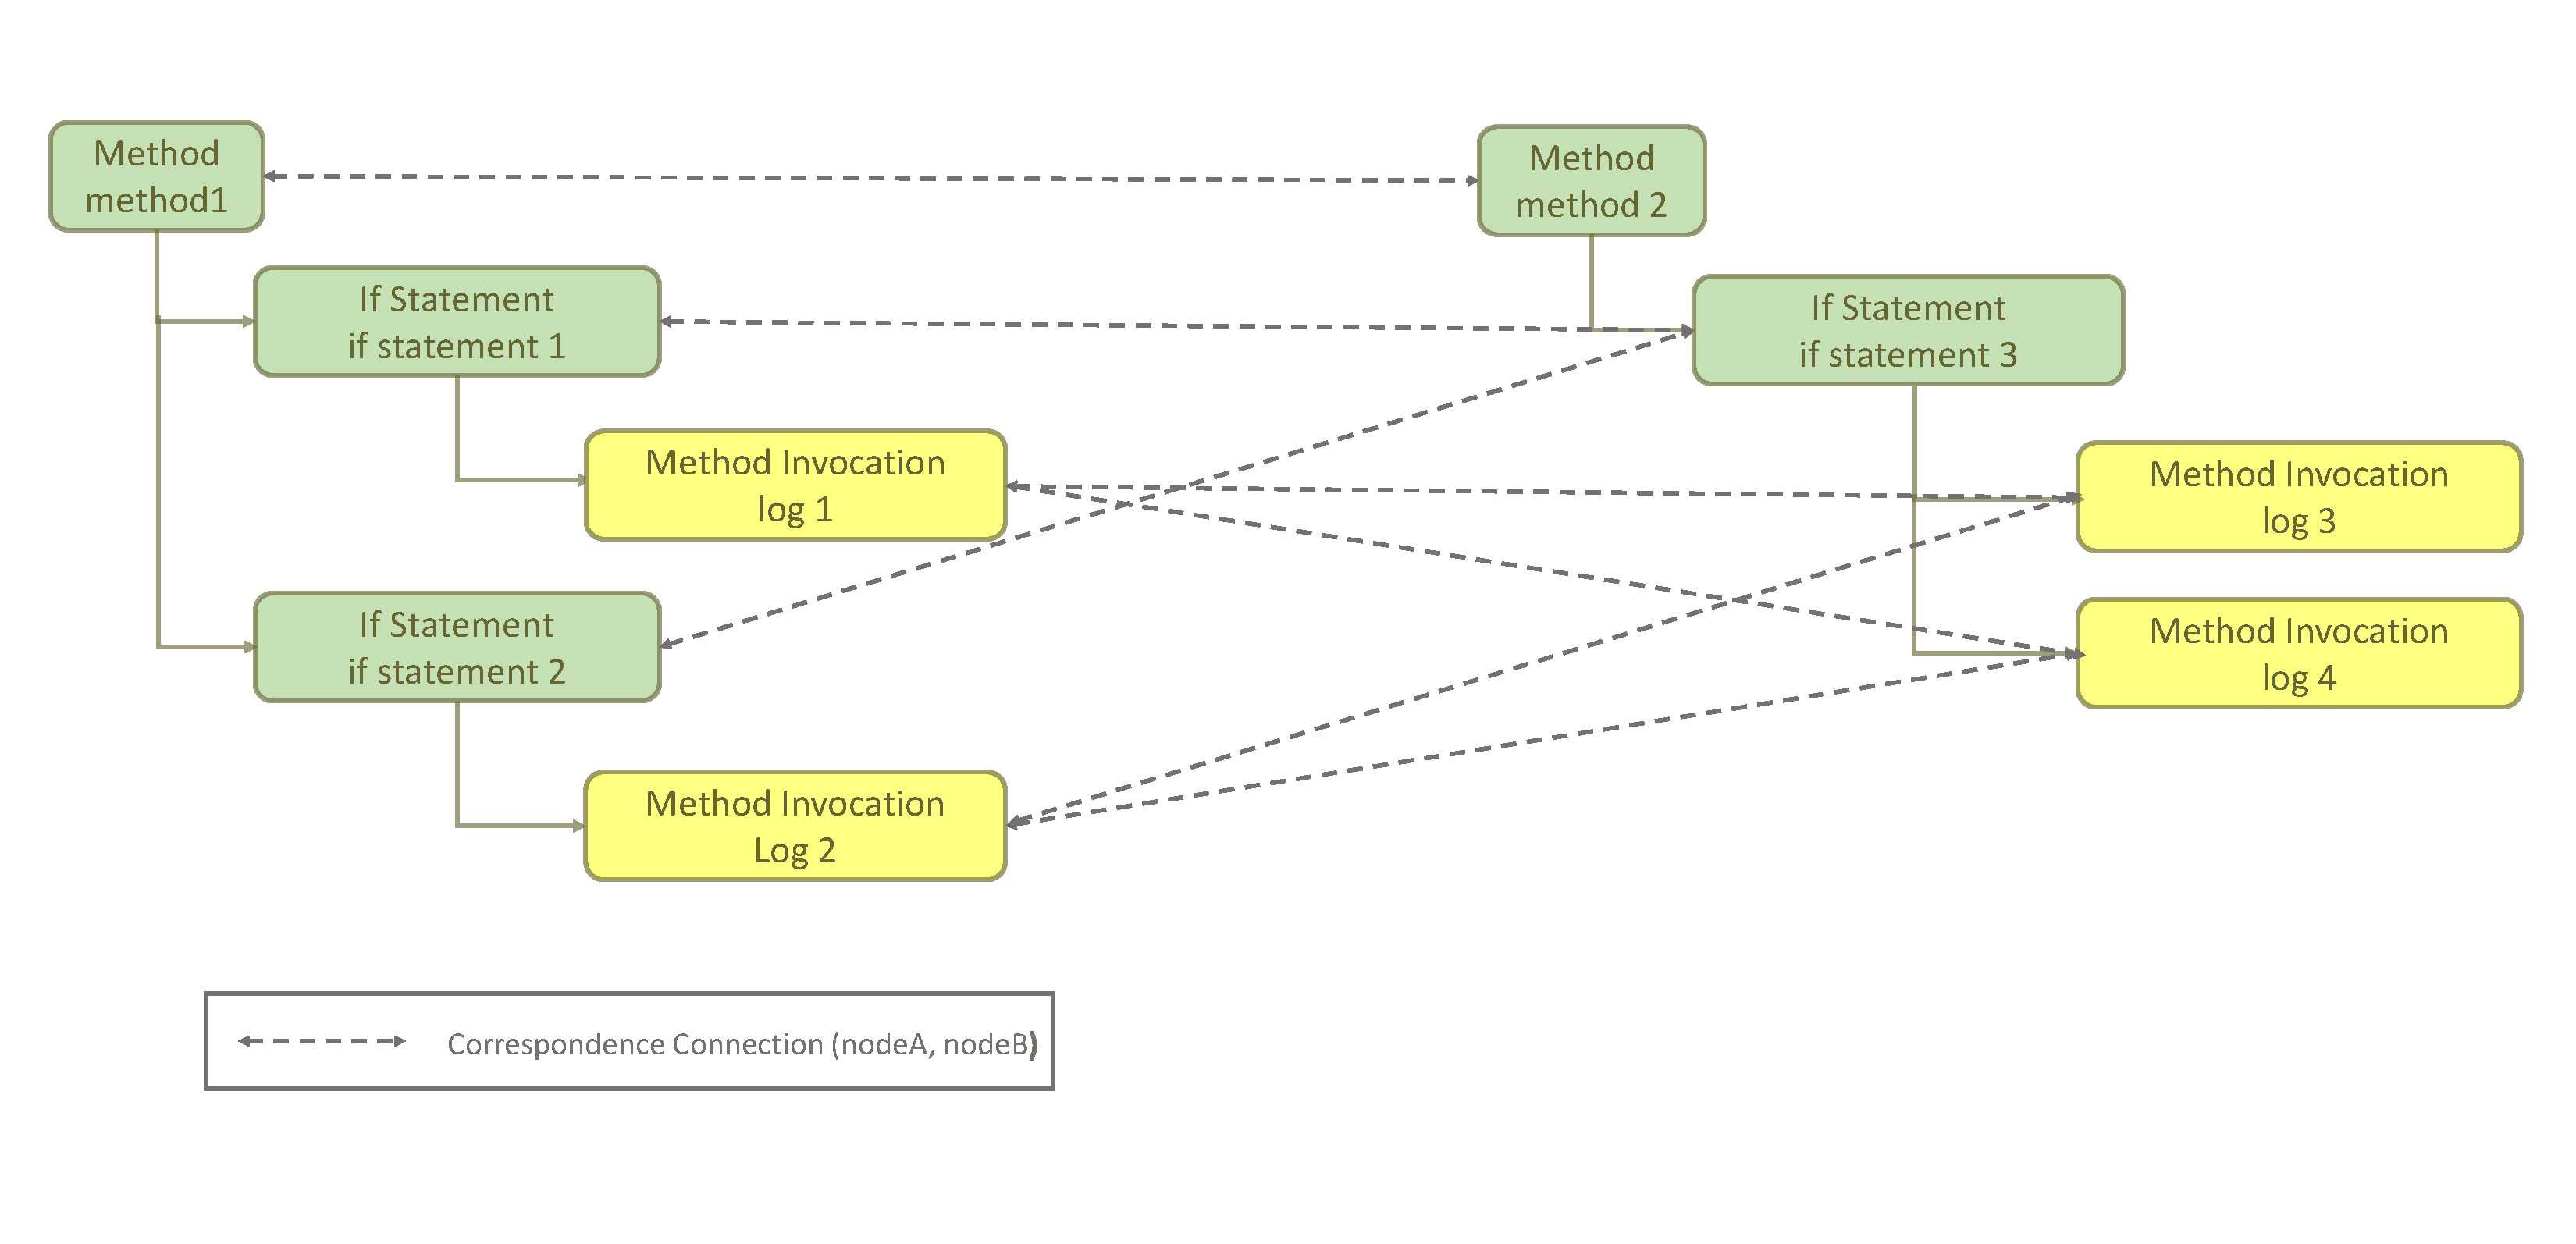
\includegraphics [width = \textwidth]{Drawing4/multipleLogging.pdf}
  \caption{Simple AUAST structure of examples in Figures~\ref{multiple1} and~\ref{multiple2}. Links between AUAST nodes indicate candidate structural correspondences detected by the Jigsaw framework.}
  \label{mast_1}
\end{figure}


\begin{figure} [H]
  \centering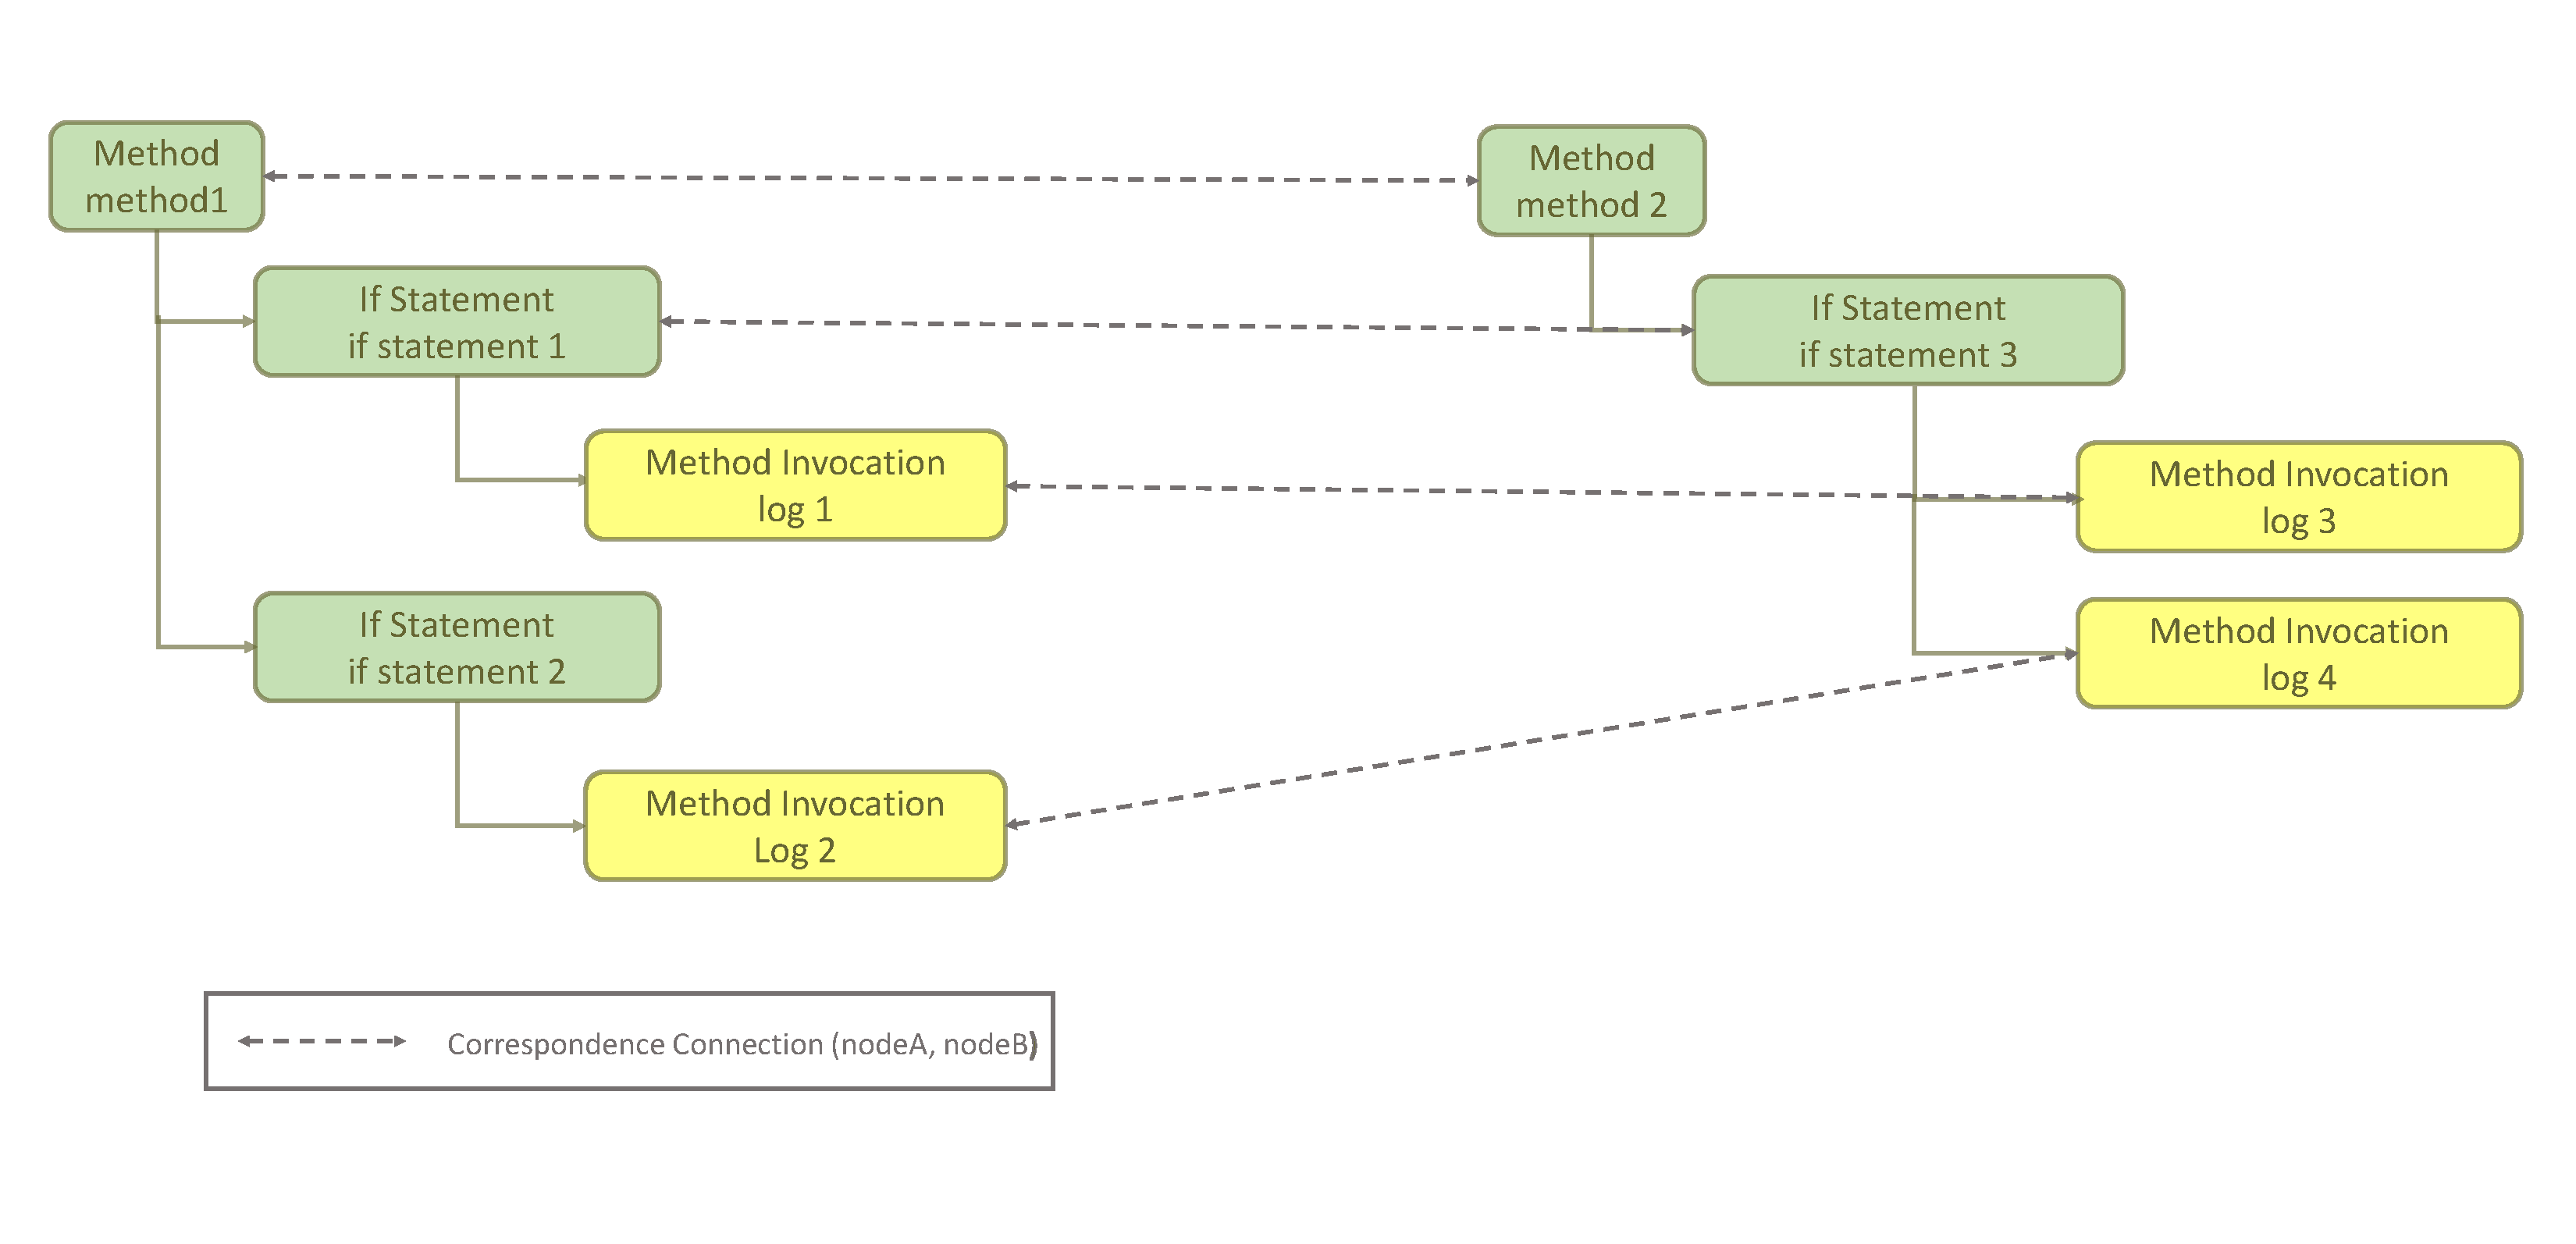
\includegraphics [width = \textwidth]{Drawing4/multipleLogging2.pdf}
  \caption{Simple AUAST structure of examples in Figures~\ref{multiple1} and~\ref{multiple2}. Links between AUAST nodes indicate structural correspondences selected as the best match using our greedy algorithm.}
  \label{m_ast2}
\end{figure}

To handle these cases, we can split them into more than one case, where each logged Java method contains only one logging call. To do so, we need to create a copy of logged Java method for each logging call by maintaining that logging call and removing the other ones. For example, we need to create two copies for each logged Java method of examples   in Figures~\ref{multiple1} and~\ref{multiple2} as depicted in Figures~\ref{multiple1-one} and~\ref{multiple2-one}, respectively.
% thus constructing four possible anti-unifier for  possible combination and compute the similarity for each combination.
%We can split this case into more than one case, each with one logging statement in every seed. That is, for each case all the other logging statements should be deleted from seeds.  For example, imagine we have AST 1 and AST 2. AST 1 contains three logging calls and AST 2 contains two logging calls. As explained, we split AST 1 into AST 1a, AST 1b, and AST 1c. Also, we split AST 2 into AST 2a and AST 2b. We can split this case into 6 possible cases and create an anti-unifier for each possible combination and then compute a measure of similarity for each case. The best match for each log statement can be selected based on anti-unifier with the highest similarity amongst the other options.


\begin{figure}[H]
\def\baselinestretch{1}
\begin{lstlisting}

public void method1(){
	...
	if(condition1){
		Log.log();
	}
	...
	if(condition2){
		//removed
	}
	...
}

public void method1(){
	...
	if(condition1){
		//removed
	}
	...
	if(condition2){
		Log.log();
	}
	...
}

\end{lstlisting}
\caption{Create multiple copies of the LJM in Figure~\ref{multiple1} for each logging call.\label{multiple1-one}}
\end{figure}



\begin{figure}[H]
\def\baselinestretch{1}
\begin{lstlisting}
public void method2(){
	...
	if(condition3){
		//removed
		Log.log();
	}
	...
}

public void method2(){
	...
	if(condition3){
		Log.log();
		//removed
	}
	...
}

\end{lstlisting}
\caption{Create multiple copies of the LJM in Figure~\ref{multiple2} for each logging call.\label{multiple2-one}}
\end{figure}
\section{An assessment of the anti-unifier-building tool}\label{anti-unifier-assessment}
%\subsection{Study 2: Detailed anti-unifier view}  \label{study2}
To assess the effectiveness of our anti-unification algorithm, we have implemented the anti-unifier-building tool, which is a plug-in to the Eclipse integrated development environment (IDE), and conducted an experiment on the test suite described in Section~\ref{jigsaw-assessment}. Our tool is developed atop Jigsaw to construct an anti-unifier for each pair of LJMs in our test suite.


\subsection{Setup}  \label{study2-setup}
In this study, we manually attempted to create the detailed anti-unifier view for each pair of LJMs in the test suite (55 test cases in total). We first identified corresponding and non-corresponding Java elements for each LJM pair with a focus on preventing the correspondence of logging calls with anything else and then represented the anti-unifier in the detailed view (i.e., formatted as in Figure~\ref{fig:meth-anti-unifier}). We also computed the ratio of common Java elements in the detailed anti-unifier view to total number of Java elements of the two LJMs to measure the similarity.  
We also ran the anti-unifier-building tool on each pair of LJM to construct the detailed anti-unifier view for each pair with special attention to logging calls and to measure the similarity between the two LJMs. Furthermore, we used \name{Eclemma}, which is a Java code coverage tool for Eclipse, to measure the test coverage. Test coverage is defined as a measure of the completeness of the set of test cases. 


%The view would be in the form depicted in ..

\subsection{Results}  \label{study2-results}
We present the results of our analysis for a subset of 10 test cases (see Table~\ref{study2_test_cases}) in Table~\ref{study2_test_cases_results}. The analysis of the output has been divided into two categories: correspondence and similarity. "Correspondence" refers to the number of corresponding lines-of-code (LOC) detected by our tool that were found to be corresponded by our manual examination as well, and the number of LOC detected as corresponded by our tool but were not found to be corresponded in our manual inspection. We also present the percentage of the correct corresponding LOC to the total number of LOC of the two LJMs. "Similarity" refers to the similarity that is computed based on the the detected correspondences. It is calculated using both our tool and manual experiment.


In Test Case 8, \name{rootEntry} method contains a nested \code{if- }statement enclosing a logging call and \name{actionPerformed} method contains an \code{if-} statement enclosing another logging call. The analysis showed that a correct correspondence was detected between the inner \code{if- }statement inside the nested \code{if} and the single \code{if-} statement. Test Cases 3 and 10 contain statements that are not found to be corresponded by our tool even though correspondences exist. For example, in Test Case 3, \name{isSupportedEncoding} method contains an assignment statement enclosed by an \code{if-} statement that does not have any correspondences and \name{send} method contains another assignment statement inside a \code{for-} statement without any correspondences as well. However, no correspondence was detected between the two assignment statements since their parent nodes are not corresponded.    

\begin{figure}
  \centering
  \begin{tabular}{|c|l|}
    \hline
    Test case & Logged Java methods \\
    \hline
    
    \multirow{2}{*}{{1}}&org.gjt.sp.jedit.PluginJAR.generateCache()\\
    \cline{2-2}
                         &org.gjt.sp.jedit.PluginJAR.generateCache()\\
    \hline
  
    \multirow{2}{*}{2}&org.gjt.sp.jedit.PluginJAR.generateCache()\\
    \cline{2-2}
                         &org.gjt.sp.jedit.EditBus.send(...)*\\
    \hline
    \multirow{2}{*}{3}&oorg.gjt.sp.jedit.MiscUtilities.isSupportedEncoding(...)\\
    \cline{2-2}
                         &org.gjt.sp.jedit.EditBus.send(...)\\
    \hline
    \multirow{2}{*}{4}&org.gjt.sp.jedit.EditBus.send(...)\\
    \cline{2-2}
                         &org.gjt.sp.jedit.EditBus.send(...)*\\
   \hline
   \multirow{2}{*}{5}&org.gjt.sp.jedit.EditBus.send(...)*\\
   \cline{2-2}
                         &org.gjt.sp.jedit.EditAction.Wrapper.actionPerformed(...)\\
 \hline
    \multirow{2}{*}{6}&org.gjt.sp.jedit.EditBus.send(...)*\\
   \cline{2-2}
                         &org.gjt.sp.jedit.BufferHistory.RecentHandler.doctypeDecl(...)\\
 \hline
    \multirow{2}{*}{7}&org.gjt.sp.jedit.EditAction.Wrapper.actionPerformed(...) \\
    \cline{2-2}
                         &org.gjt.sp.jedit.JARClassLoader.loadClass(...)\\
 \hline
    \multirow{2}{*}{8}&org.gjt.sp.jedit.EditAction.Wrapper.actionPerformed(...) \\
    \cline{2-2}
                         &org.gjt.sp.jedit.io.VFS.DirectoryEntry.RootsEntry.rootEntry(...)\\
 \hline
    \multirow{2}{*}{9}&org.gjt.sp.jedit.PluginJAR.generateCache()\\
    \cline{2-2}
                         &org.gjt.sp.jedit.BufferHistory.RecentHandler.doctypeDecl(...)\\
 \hline
    \multirow{2}{*}{10}&org.gjt.sp.jedit.io.VFS.DirectoryEntry.RootsEntry.rootEntry(...)\\
    \cline{2-2}
                         &org.gjt.sp.jedit.ServiceManager.loadServices(...) \\
  \hline
 
  \end{tabular}
  \caption{10 sample logged Java method pairs used as test cases.}
  \label{study2_test_cases}
\end{figure}

 
\begin{figure}
  \centering
  \begin{tabular}{|c|c|c|c|c|c|}
    \hline
    \multirow{2}{*}{Test case}&\multicolumn{2}{c|}{Correspondence}&\multicolumn{2}{c|}{Similarity}\\
    \cline{2-5}
    &Correct (\%)&Incorrect&human&tool\\
    \hline
    1&104(100)&0& 1.0 & 1.0\\
    \hline
    2&8(100)&0& 0.13& 0.13\\
    \hline
    3&6(85)&1&0.19& 0.16\\
    \hline
    4&4(100)&0&0.29 &0.29\\
    \hline
    5&5(100)&0&0.21 &0.21\\
    \hline
    6&3(100)&0&0.2 &0.2\\
    \hline
    7&5(100)&0&0.11 &0.11\\
    \hline
    8&7(100)&0& 0.1&0.1\\
    \hline
    9&3(100)&0&0.03&0.03 \\
    \hline
    10&14(87)&2&0.27 &0.22\\
    \hline
   
  \end{tabular}
  \caption{Results of constructing anti-unifiers with a focus on logging calls for the 55 test cases.}
  \label{study2_test_cases_results}
\end{figure}
 
The results of the pairwise comparison between LJMs of the test suite is visualized in Figure~\ref{fig:au_graph}. Our anti-unifier-building tool succeeded in detecting correspondences with special attention to anti-unifying logging calls and calculating pairwise similarities in 48 out of 55 test cases. In addition, the test coverage of our test cases was measured 82\% using \name{EclEmma}.

\begin{figure} [H]
  \centering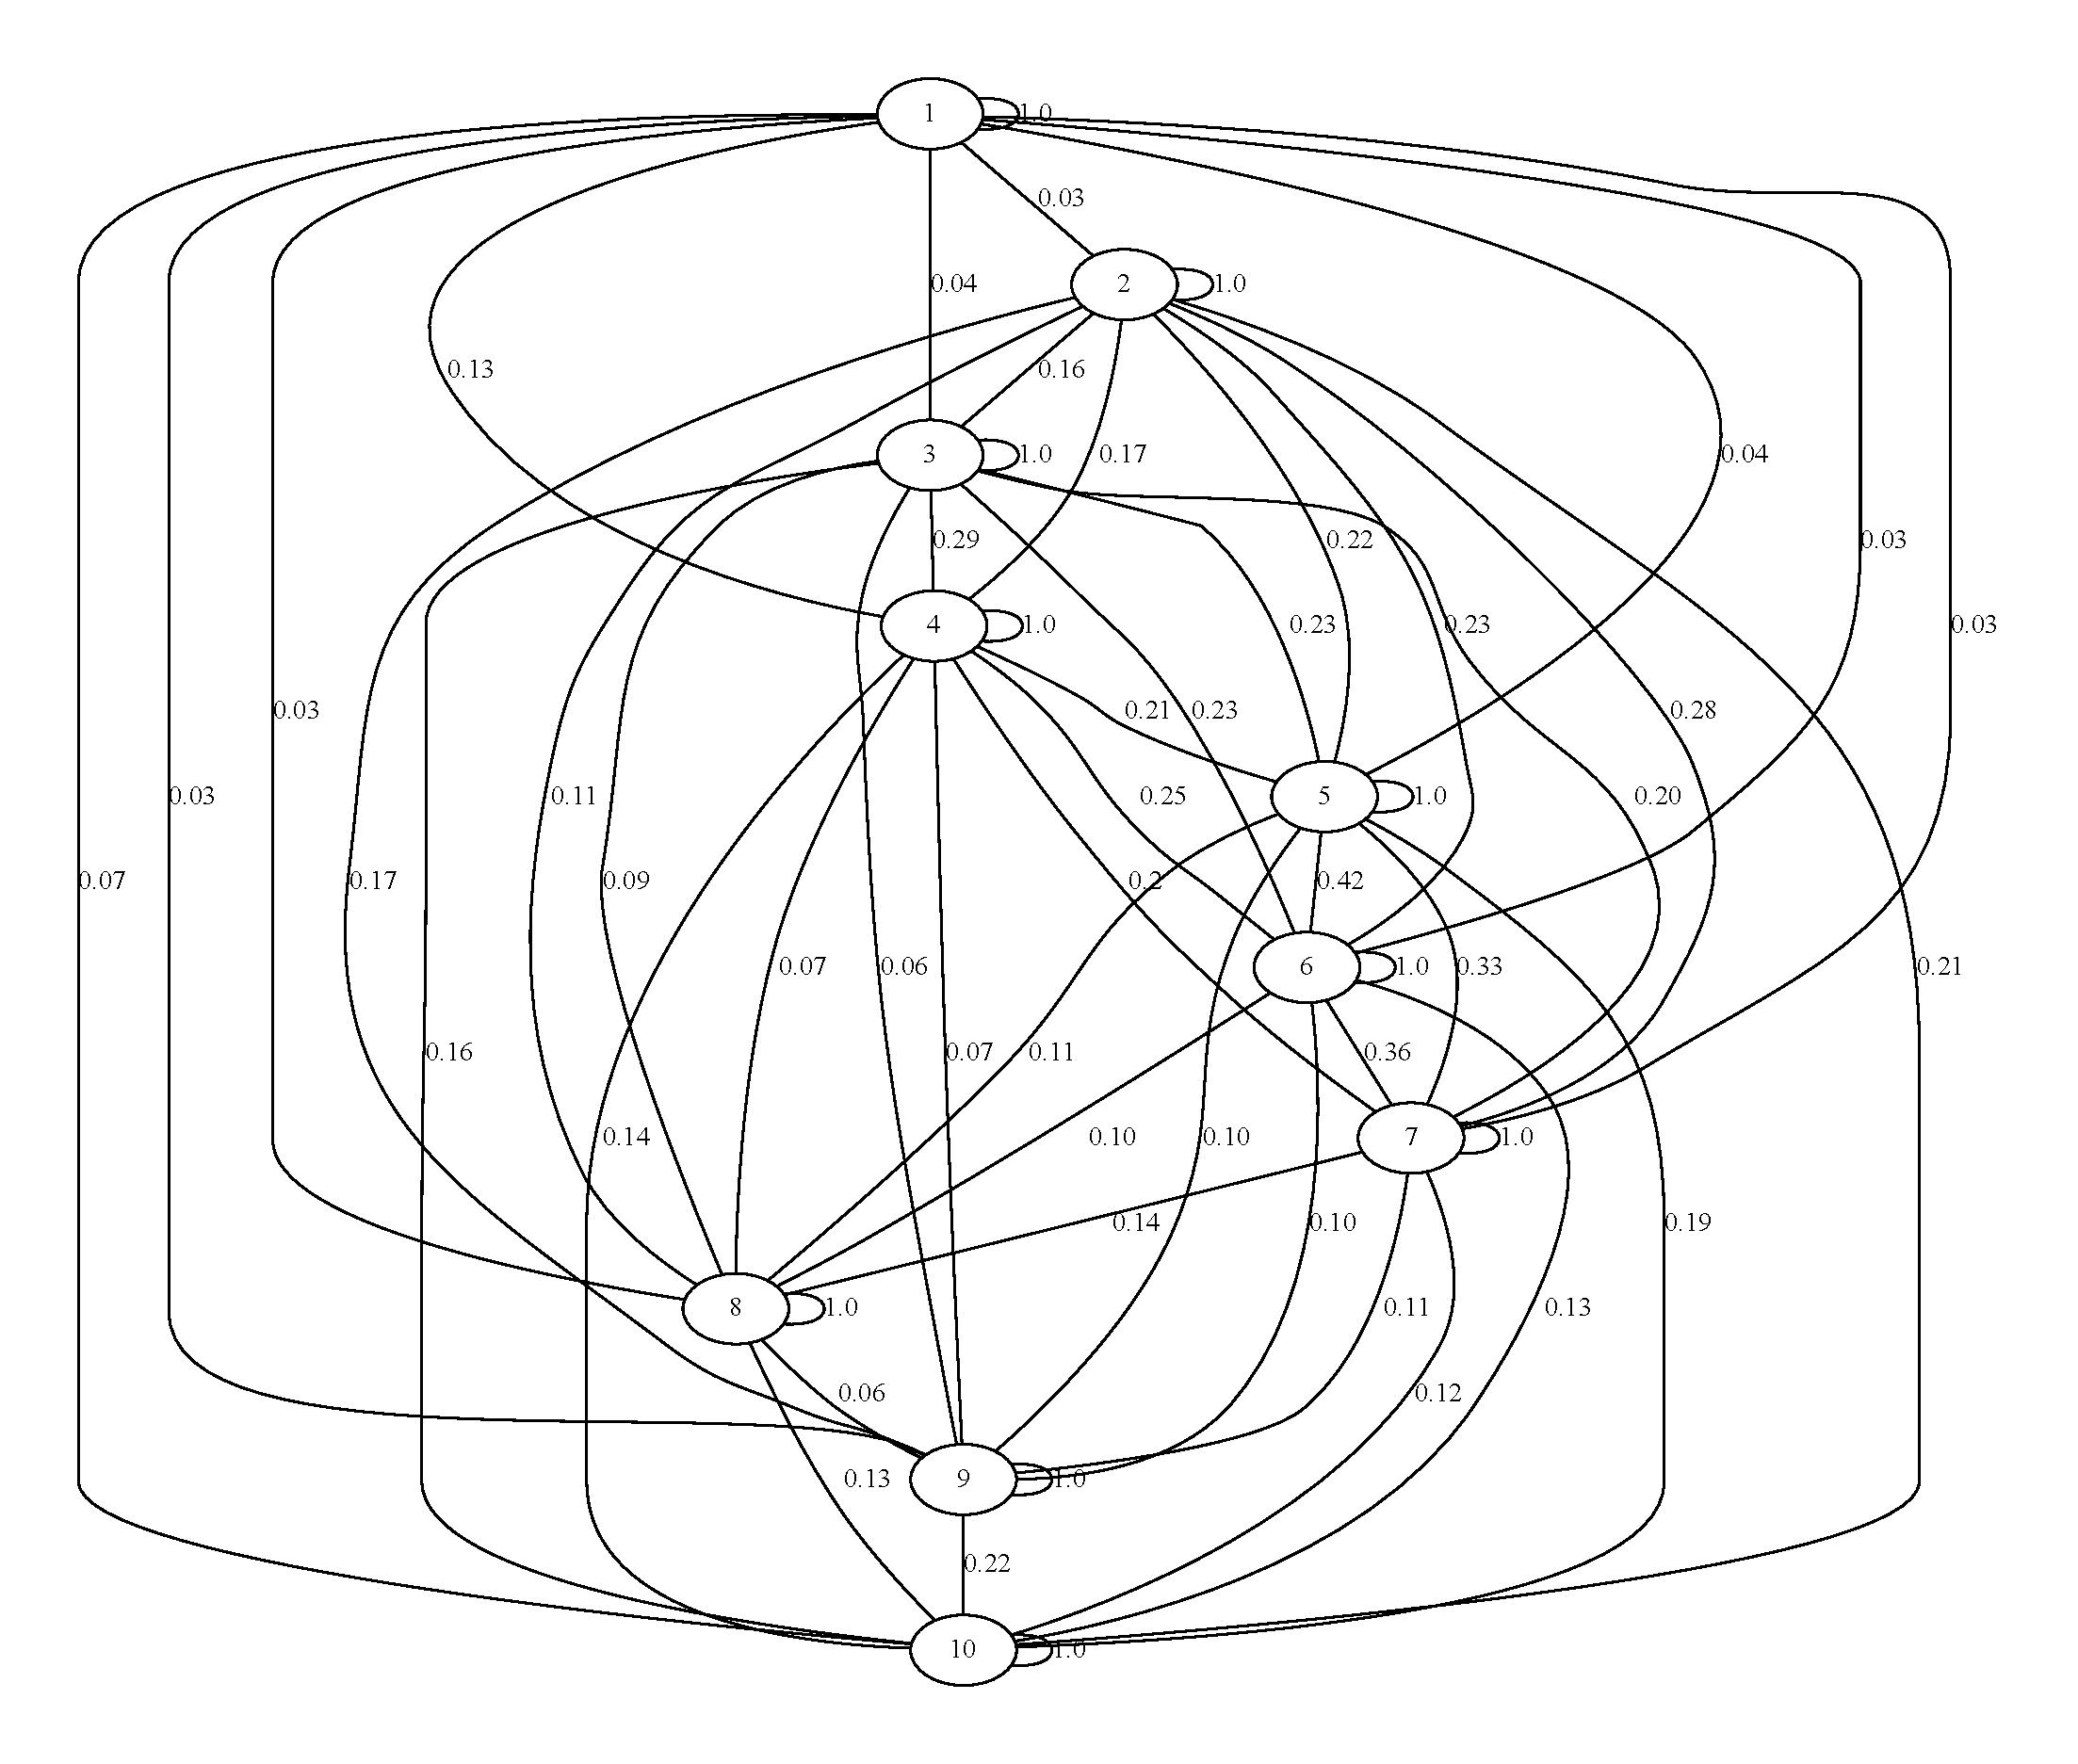
\includegraphics [width = \textwidth]{graphviz/au.pdf}
  \caption{A similarity graph representing pairwise similarities calculated by our tool between LJMs shown in Table~\ref{table:ljms}.}
  \label{fig:au_graph}
\end{figure}


\section{Summary} \label{meth1-summary}
We have presented an approach for constructing a generalization from ASTs of two logged Java methods with special attention to logging calls. This approach is implemented as an Eclipse plug-in which given two logged Java methods utilizes the Eclipse JDT framework to extract their ASTs. In order to be able to apply HOAUMT, we extended the AST structure to a higher-order structure, called AUAST, that would allow the insertion of variables in place of any nodes. We then applied the Jigsaw framework to identify potential correspondences between the two AUASTs and greedily determines the best correspondence for each node with the highest Jigsaw similarity.  Moreover, some constraints have been applied on the selection of correspondences to prevent anti-unifying log method invocation nodes with any other types of node. The anti-unification of two AUASTs is performed through the application of higher-order modulo theories over the AUAST structures. A measure of similarity has been developed that would provide us with useful information for the clustering phase. Furthermore, an empirical study was conducted to evaluate the effectiveness of our anti-unification algorithm and the anti-unifier-building tool in constructing an anti-unifier from each LJM pair of our test suite with special attention to logging calls and measuring similarity between them.  
